\documentclass[a4paper,12pt,english]{article}\usepackage[]{graphicx}\usepackage[]{xcolor}
% maxwidth is the original width if it is less than linewidth
% otherwise use linewidth (to make sure the graphics do not exceed the margin)
\makeatletter
\def\maxwidth{ %
  \ifdim\Gin@nat@width>\linewidth
    \linewidth
  \else
    \Gin@nat@width
  \fi
}
\makeatother

\definecolor{fgcolor}{rgb}{0.345, 0.345, 0.345}
\newcommand{\hlnum}[1]{\textcolor[rgb]{0.686,0.059,0.569}{#1}}%
\newcommand{\hlsng}[1]{\textcolor[rgb]{0.192,0.494,0.8}{#1}}%
\newcommand{\hlcom}[1]{\textcolor[rgb]{0.678,0.584,0.686}{\textit{#1}}}%
\newcommand{\hlopt}[1]{\textcolor[rgb]{0,0,0}{#1}}%
\newcommand{\hldef}[1]{\textcolor[rgb]{0.345,0.345,0.345}{#1}}%
\newcommand{\hlkwa}[1]{\textcolor[rgb]{0.161,0.373,0.58}{\textbf{#1}}}%
\newcommand{\hlkwb}[1]{\textcolor[rgb]{0.69,0.353,0.396}{#1}}%
\newcommand{\hlkwc}[1]{\textcolor[rgb]{0.333,0.667,0.333}{#1}}%
\newcommand{\hlkwd}[1]{\textcolor[rgb]{0.737,0.353,0.396}{\textbf{#1}}}%
\let\hlipl\hlkwb

\usepackage{framed}
\makeatletter
\newenvironment{kframe}{%
 \def\at@end@of@kframe{}%
 \ifinner\ifhmode%
  \def\at@end@of@kframe{\end{minipage}}%
  \begin{minipage}{\columnwidth}%
 \fi\fi%
 \def\FrameCommand##1{\hskip\@totalleftmargin \hskip-\fboxsep
 \colorbox{shadecolor}{##1}\hskip-\fboxsep
     % There is no \\@totalrightmargin, so:
     \hskip-\linewidth \hskip-\@totalleftmargin \hskip\columnwidth}%
 \MakeFramed {\advance\hsize-\width
   \@totalleftmargin\z@ \linewidth\hsize
   \@setminipage}}%
 {\par\unskip\endMakeFramed%
 \at@end@of@kframe}
\makeatother

\definecolor{shadecolor}{rgb}{.97, .97, .97}
\definecolor{messagecolor}{rgb}{0, 0, 0}
\definecolor{warningcolor}{rgb}{1, 0, 1}
\definecolor{errorcolor}{rgb}{1, 0, 0}
\newenvironment{knitrout}{}{} % an empty environment to be redefined in TeX

\let\hlstd\hldef
\let\hlstr\hlsng
\usepackage{alltt}
% \usepackage[paperwidth=164mm, paperheight=280mm, top=19mm, bottom=19mm, left=1cm, right=1cm]{geometry} % 16:9 three pages in a row
\usepackage[outer=4cm, inner=3cm, marginparwidth=3cm, marginparsep=0.5cm]{geometry}
\usepackage[english,provide=*]{babel}
\usepackage{longtable}
\usepackage{array}
\usepackage{fontspec}
\usepackage{booktabs}
\usepackage{hyperref}
\usepackage{varioref} %% vref
% \usepackage{paralist} %% compactenum %% Not available on ALVIS
% \usepackage{siunitx} %% \num %% Not available on ALVIS
% \usepackage{IEEEtrantools} % proper indentation for multi-line equations %% Not available on ALVIS
\usepackage{amsmath} %% \pmatrix
% \usepackage{subfig} %% Not available on ALVIS
% \usepackage{apacite} %% Not available on ALVIS
% \usepackage[framemethod=tikz]{mdframed} % nice textboxes %% Not available on ALVIS

%% make a single « start and end a chunk of \texttt{}, and two «« to represent the literal «.
\catcode`«=\active
\def«#1«{\texttt{#1}}
\IfFileExists{upquote.sty}{\usepackage{upquote}}{}
\begin{document}

\title{Intimate partner violence in low- and middle-income countries \\
  \large What neighbours think and spouses do
}

\author{
  \IEEEauthorblockN{Björn Halleröd}
  \IEEEauthorblockA{Dept. of Sociology and Work Science\\
    University of Gothenburg\\
    Sweden
    bjorn.hallerod@gu.se}
  \and
  \IEEEauthorblockN{Hans Ekbrand}
  \IEEEauthorblockA{Dept. of Sociology and Work Science\\
    University of Gothenburg\\
    Sweden
    hans.ekbrand@socav.gu.se}
  \IEEEauthorblockN{Mary Zhang}
  \IEEEauthorblockA{Department of Social Policy, Sociology and
    Criminology, School of Social Policy and Society \\
    University of Birmingham \\
    f.zhang.4@bham.ac.uk}
}

\author{
  \large Björn Halleröd (bjorn.hallerod@gu.se), University of Gothenburg \and
  \large Hans Ekbrand (hans.ekbrand@socav.gu.se), University of Gothenburg \and
  \large Mary Zhang (f.zhang.4@bham.ac.uk), University of Birmingham
}

% \institution{University of Gothenburg}

% * Correspondence:
% \href{mailto:bjorn.hallerod@socav.gu.se}{\nolinkurl{bjorn.hallerod@socav.gu.se}},
% Department of Sociology and Work Science, University of Gothenburg, Box
% 720, Göteborg, Sweden, 40530


\maketitle


% Abstract

% {[}TBC{]}

% \textbf{Keywords:} intimate person violence; domestic violence; human
% rights; low- and middle-income countries


\section{Introduction}
\marginpar{\small Slightly rephrased to emphasize that the context is our main focus.}
In this article we will analyse factors that influence
women's risk of experiencing intimate partner violence (IPV). We will
pay special attention to the social context in which IPV takes place,
specifically the level of gender equality in the country and the
attitudes to IPV in the local neighbourhood.

Recent estimates indicate that more than one-fifth of the world's women
who are or have been living in a partnership have experienced IPV. The
risk of IPV is highest among younger women and among mothers with caring
responsibilities (Sardinha et al., 2022). IPV is a grave human rights
violation with serious negative and sometimes mortal consequences for
women (Beyer et al., 2015; Devries et al., 2013; Elvin-Nowak et al.,
2023; Stockl et al., 2013) and also has negative impact on their
children (Rawlings \& Siddique, 2020; Schrubbe et al., 2023). Still, a
large proportion of women justify husbands' use of violence. In
fact, our calculations of data from the Demographic and Health Survey
(DHS) in most low- and middle-income countries (LMICs) shows that the
proportion of women justifying IPV, or wife beating as it is called in
the questionnaires, not only is larger than the proportion of men
justifying IPV, but also clearly higher than the proportion of women who
have been exposed to IPV. There is also a strong positive correlation
between women's acceptance of IPV and women's risk of experiencing IPV.
Women who are beaten are more likely to view their husbands' use of
violence as justifiable (Haque et al., 2022). We want to emphasize from
the outset that we do not view women's justification of IPV as a cause
of IPV. It is possible that women's acceptance of IPV lowers the
barriers for husbands to use violence. Still, this acceptance is just as
likely an ex-post justification of experienced IPV (Eckstein, 2011).

\marginpar{\small Recasted according to the new framing.}
Moving away from the individual spouse, it is important to shed light
on if and how acceptance of IPV among women in the neighbourhood
correlates with the individual risk among women to be exposed to IPV.
Broad acceptance of IPV in a neighbourhood indicates disempowerment of
women which should make women more exposed to IPV. By careful use of
geolocated survey data we can measure the proportion of women in the
local neighbourhood who thinks IPV can be justified, and investigate
what predictive power this factor has on IPV.

\marginpar{\small ``predictive power'' and ``association'' when speaking of the ``effect'' of the attitudes in local area.}
Taking a step further in describing the context of IPV, we can combine
the attitudes toward IPV of the wife and the husband, classify couples
accordingly, and investigate if these attitudes moderate the
association between the attitudes of women in the neighbourhood
and the individual woman's risk if IPV.

\marginpar{\small ``predictive power'' when speaking of the ``effect'' of gender equality.}
In the same vein, we will also analyse the predictive power of gender
equality at a societal level on women's risk of being exposed to IPV.
Again, the attitudes toward IPV in the couple might moderate the
predictive power between gender equality at the societal level and
IPV.

In a broader sense, we want to better understand how beliefs affect
the link between the social context and individual actions. To address
this issue, we use a survey-based sample that covers 42 low- and
middle-income countries and 32 Indian states, utilising multilevel
information from women, spouses, neighbours, and countries.

Our outcome is women's risk of experiencing IPV by her current partner.
We relate that to women's justification of husbands' right to use
violence. We also include the husband's attitudes towards IPV, whether
he considers the use of IPV justifiable or not. This approach allows us
to analyse not only how the husband's views on IPV are linked to his
actions but also to explore the spouses' combined views, i.e.,
agreements and disagreements between spouses. Moreover, we incorporate
the extent to which women in the neighbourhood justify IPV. Since our
data are compiled from several countries, we also use data on
country-level gender equality. Hence, we can address whether, in social
settings where women generally hold a stronger position, the risk of IPV
decreases, regardless of the spouses' views on IPV and the attitudes of
neighbours.

This study contributes to the research field in several ways: First,
husbands are often absent in the literature. By using data on
attitudes towards IPV and empowerment from both spouses, we deepen the
understanding of women's disempowerment and the importance of
attitudes related to IPV. Our second main contribution is the
systematic integration of neighbourhood and country effects into the
analyses to understand IPV as a social phenomenon, i.e., the fact that
spouses do not live in a social vacuum. Finally, we will elucidate if
and to what degree the attitudes of the couple moderates the link
between the social context and the actions of the individual. \marginpar{\small recasted to fit the new framing.}

\section{Background}
As mentioned, acceptance of IPV among women is strongly correlated with
their experience of actual IPV. We find it likely that in the individual
case, there could be a causal relationship between experienced IPV and
justification of IPV, but that the direction of the causality varies
between individuals and possibly also within individuals over time.
Women blaming themselves for being beaten, afterwards justifying their
husbands' behaviour, is a well-known phenomenon (Flood \& Pease, 2009;
Lelaurain et al., 2021; Luke et al., 2007; Wood, 2001). However, the
opposite causality could also be the case (Uthman, Lawoko, et al.,
2009), as IPV justification might lower the hurdles for husbands to use
violence and lower women's likelihood to protest against the use of IPV.
Hence, in accordance with previous research, we expect a correlation,
but we do not assume it is a one-directional causation.

Regardless of the causes, women's acceptance of IPV is a strong
indicator of disempowerment, acknowledging husbands' right to use
physical violence to enforce their will and exercise control (Eze-Ajoku
et al., 2022; Heaton \& Forste, 2008). This is also reflected in the way
data on IPV are collected. For example, in the DHS, questions about the
justification of IPV are related to how the wife handles household
chores and child-rearing, women's right to leave the home without
telling the husband, and their right to refuse sex (see Table 1). Hence,
the justification of IPV is tied to aspects central to the discussion of
women's empowerment (Cunningham et al., 2015; Pratley, 2016). Women are
generally considered empowered when they participate in decision-making
related to themselves, the household, and intimate relationships. That
includes involvement in economic decision-making concerning purchases,
health care, having and exercising control over one's income, savings,
and so on. In addition, empowerment often has a social dimension: women
are empowered if they control with whom they socialise, participate in
social activities, and are allowed to leave home without the husband's
consent (Carlson et al., 2015; Cunningham et al., 2015; Machio et al.,
2022). So, even though attitudes towards or experience of IPV are
usually not directly included in the concept or measurement of women's
empowerment, there is a direct link between justification of IPV and
disempowerment of women.

If the husband thinks IPV can be justified, it likely increases the
probability that he has used violence against his wife. Also, in the
case of husbands, it is reasonable to assume a causality between the
justification of IPV and the use of IPV. But again, the causation can
go in both directions. Some husbands use violence because they think
it is just; others afterwards justify why they beat their wives
(Eckstein, 2011). Somewhat counterintuitively, the correlation between
the husband's, or the perpetrator's, attitudes towards IPV and the
wife's risk of experiencing IPV tend to be lower compared to the
correlation between the wife's attitudes to IPV and her experience of
IPV (c.f., Arefaynie et al., 2021; Chowdhury \& Mathur, 2021; Krause
et al., 2016; Patil \& Khanna, 2022). However, spouses' attitudes to
IPV should reasonably be understood from a relational perspective. If
both husband and wife agree that IPV is unjustifiable, the IPV risk is
likely low. But what if they agree that the husband has the right to
use violence? Given what we know about the correlation between
attitudes towards and use of IPV, it is reasonable to assume that the
IPV risk is high. On the other hand, it could also indicate that
spouses have a coherent set of values that lowers the risk for
conflict and possibly also the use of violence. We will also have
situations where the husband justifies IPV while the wife does not
and, more intriguing, when the victim, the wife, accepts the use of
violence, while the perpetrator, the husband, does not. To our
knowledge, large-scale survey-based analyses that include both
spouses' attitudes to IPV are missing. Our aim is to fill this gap.

\subsection{The neighbourhood and the country}
Individuals and families are embedded in the surrounding society and
confined by its normative and behavioural boundaries. These boundaries
are sometimes formal, for example, restrictions on women's access to
education or the labour market and usually decided at the country level.
Many boundaries are informal and normative prescriptive, regulating what
is socially acceptable and upheld within daily interaction within the
family, the neighbourhood and society (Coleman, 1988). We therefore
assume that women's standing in society is of importance for each
woman's empowerment, setting a collective standard for what women and
men should and can do.

In a simplistic way, the neighbourhood can affect individuals via two
main routes. Socio-economic segregation means individuals within the
same neighbourhood often share similar economic and educational
circumstances. However, neighbours are also commonly linked to social
organisation, social control, and norms. From this perspective,
developed in relation to urban settings in the United States (Sampson
et al., 2002), women in poorer neighbourhoods are more exposed to IPV
because of a lack of commonly acknowledged norms, a lack of social
control and a lack of social condemnation of the perpetrator of IPV.
It follows that condemnation of violence is assumed to be a central
part of mainstream social norms. Perpetrators of IPV will in these
cases be exposed to stigmatization (Goffman, 2009) and the knowledge
of that will have a \emph{restraining effect} on the potential use of
IPV. We assume that this restraining effect will operate regardless of
the individual's own beliefs in justifiable use of violence. However,
in some countries and even more so in local areas within countries,
the husband's right to use violence against his wife is the dominant
social norm. There are also countries and local areas where a majority
of women report that they experienced IPV. In these cases, it is
likely that norm-adjusted behaviour is not restraining but increases
acceptance of IPV (Uthman, Moradi, et al., 2009) and the occurrence of
IPV (Beyer et al., 2015; Mookerjee et al., 2022; Pinchevsky \& Wright,
2012). In these cases, we can assume that the prevailing social norm,
that is justifiable for the husband to use violence, amplifies the
importance individual beliefs about the husband's right to use
violence. Hence, to understand the importance of spouses' attitudes
towards IPV, we need to understand the social context in which these
attitudes are expressed.

\section{Expectations and Interactions}
Based on previous research, we have formulated a set of hypotheses
that test how gender equality and justifications of IPV in the
neighbourhood influences women's risk of IPV.

\begin{description}
  \marginpar{\small Reduced to hypotheses about how the social context affects the risk of IPV.}
\item[Hypothesis 1] Women living in a neighbourhood where IPV is
  widely accepted suffer from an increased IPV risk. Hence,
  neighbours' attitudes are supposed to have an independent
  association with the husband's use of violence against the wife even
  under control for the attitudes in the couple.
\item[Hypthesis 2] Net of spouse's and neighbours' justification of
  IPV, the IPV risk is lower in countries that are more gender equal.
\end{description}

In addition to these hypotheses, we also investigate if the attitudes of
the couple moderate the effects spelled out in the two hypotheses.

\begin{description}
  \marginpar{\small Recasted to fit the new framing, but both
    perspective on the interaction are taken.}
\item[Interaction 1] The association between the level of the
  acceptance of IPV in the local neighbourhood and the risk of IPV may
  be moderated by the attitudes of the couple. Perhaps the association
  is stronger in couples where both spouses justifies IPV and weaker
  in couples where none of the spouses think IPV can be justified.

  Or, put the other way around, the correlation between justifications
  of IPV in the couple and the risk for the woman to be exposed to IPV
  might vary depending on the kind of local neighbourhood they live
  in.

  We anticipate that the association between spouses' justification of
  IPV and the wife's risk of being exposed to IPV is amplified in
  neighbourhoods where IPV is widely accepted.

  In the same vein, we expect that living in a neighbourhood where few
  accept IPV has a restraining effect and weakens the association
  between spouses' acceptance of IPV and wives' IPV risk.

  % We do not assume that the interaction effect has to be linear. We
  % expect the marginal effect to be weak in the lower end of the
  % distribution, i.e., when most neighbouring women condemn IPV and in
  % the upper end of the distribution when IPV is widely accepted among
  % neighbours. Hence, we expect the strongest interaction effect in the
  % lower and upper end of the distribution of neighbours' acceptance of
  % IPV, restrained in the lower end and amplified in the upper end.

\item[Interaction 2] We expect that the association between gender
  equality at the country level and IPV against the wife is stronger
  in couples where both spouses accepts IPV and weaker in couples
  where none of the spouses accepts IPV.
\end{description}



\section{Data, Variables, and Modelling}
We start with DHS data collected between 2013 - 2022 that include the
women's domestic violence module, included in the DHS IR files. The
domestic violence module was used in 44 countries, and 1,029,805 women
responded to the module. We used these data to derive the neighbourhood
variable for women's justification of IPV. Questions about the
experience of IPV were only asked to a sub-section of the sample, which
leaves 429,060 respondents. In all 44 countries, DHS also include a male
domestic violence module, included in the DHS MR files, compiling data
from 489,920 men. The smaller sample is the reason we refrained from
estimating neighbourhood acceptance of IPV for men. The female and male
data sets were merged, and only households where both spouses were
interviewed and properly matched were kept. Given these restrictions, we
end up with a working data set of 294,583 households. Because of the
size and huge variation within India, we have chosen to treat Indian
states as countries, meaning that we have 68 country units, 36 countries
and 32 Indian states\footnote{The administrative units of India have
  changed slightly over time. We use, with two minor amendments the
  standard applied by GDL. The union territories Chandigarh is merged
  with Punjab and the island group Lakshadweep is merged with Kerala.}.
We gather our country-level data on Gross Domestic Product per capita
(GDP/pc) and gender equality index (GDI) from the Global Data Lab that
provide regional data that allow us to distinguish between the Indian
states.

\subsection{Main variables}
DHS asks eleven questions, to women only, about the experience of IPV that are
summarised into three categories: less sever, sever, and sexual
violence. The gradation between less severe and severe violence appears
to some degree arbitrary. We therefore use any physical IPV as our main
indicator while validating the results using the three DHS categories
one by one.

Both spouses are asked if IPV is justifiable given five
circumstances specified in Table 1. If an individual, i.e., one of the
spouses, justify IPV in any of the five circumstances, he or she is
coded as an individual that justify the husbands right to use IPV. We
have merged the answers from each spouse into four categories, capturing
the couple's attitudes.

DHS bases each national sample frame on two steps. First, a
geographical cluster is selected, and secondly, several households are
randomly selected within each cluster. For each woman in each sampling
cluster, we have calculated the proportion of ``cluster-neighbours''
that justifies IPV. The attitude of the woman in question is not
included in those calculations, which makes the attitude of the couple
independant from the attitudes in the neighbourhood: even when 100\%
of women in the neighbourhood justify IPV, in any particular couple
the woman can have any attitude.

Our main country-level indicator is the GDL's Sub-national Gender
Development Index (GDI). The GDI is put together from three main
components: education, health and standard of living. Separate indexes
have been calculated for men and women, and the GDI is created by
dividing the female index by the male index (Global\_Data\_Lab, 2024).
Lower values indicate that women are at a disadvantage compared to
men. Because GDI is sub-national, we get unique estimates for each
Indian state.

See Table 1 in the appendix for more information on substantive
information, variable names, and the DHS variables used to derive the
variables using the original DHS-names.

\subsection{Control variables}
Women's empowerment is related to other household members, in
particular, the husband's decision powers (Luke et al., 2007). The best
solution seems to be spousal cooperation and joint decision-making
(Singh et al., 2014; Uthman, Moradi, et al., 2009). We have added two
variables which include information from both spouses to control
for decision-making related to large household purchasing and the wife's
healthcare. Education is included as a socioeconomic indicator because
of the basic assumption that more education increases the individual
room for agency both within and outside the household. Education is also
consistently associated with lower levels of IPV (Devries et al., 2013).
Again, we incorporate a relational component, constructing an indicator
that measures the husband's relative education, i.e., whether it is
higher, lower, or equal to the wife's education. Detrimental living
conditions and poverty increase the risk and acceptance of IPV
(Eze-Ajoku et al., 2022; Park et al., 2024; Sado et al., 2014; Uthman,
Lawoko, et al., 2009). We use the international wealth index (IWI), an
internationally comparable measure that indicates a household's
possession of a basic set of assets valued highly by people across the
globe (Smits \& Steendijk, 2015), to measure the households' access to
economic resources. IWI was developed by the Global Data Lab, which also
provides the code for deriving IWI from DHS data. We control for the
wife's age, given that the older she is, the longer her IPV exposure
time. The number of children is both an economic and workload indicator
possibly related to the wife's IPV risk. Finally, we control for gross
national income per capita (GDP/pc) with unique values for countries and
Indian states.

\subsection{Some descriptive data about the sample}
Table 2 shows the distribution of the variables used in the regression
models, and in the leftmost column, which variable in the regression
models they correspond to. Almost 29 per cent of wifes reported having
being exposed to IPV by their current husband.

In 48 per cent of the cases, none of the spouses justify IPV, while in
almost 15 per cent, both spouses see it as acceptable under some
circumstances. However, there is also substantial intra-household
disagreement; in 37 per cent of households, the husband and wife had
divergent views.

\begin{longtable}[]{@{}llll@{}}
\toprule 
Var  & Description & Per cent & Std. \\
\midrule
\endhead
$y$ & Wife experienced IPV & 28.6 & \\
& & & \\
& None of the spouses justifies IPV & 48.3 & \\
$x_1$ & Only Wife justifies IPV & 24.5 & \\
$x_2$ & Only Husband justifies IPV & 12.4 & \\
$x_3$ & Wife \& Husband justify IPV & 14.8 & \\
& & & \\
$x_4$ & Proportion of women in neighbourhood accepts IPV & 0.39 & 0.29 \\
$x_5$ & Gender Equality Index, normalized & 0.65 & 0.20 \\
& & & \\
& Joint decisions on healthcare & 30.6 & \\
$x_6$ & Agree - wife decides & 2.1 & \\
$x_7$ & Agree - husband decides & 13.3 & \\
$x_8$ & Don't agree & 54.1 & \\
& & & \\
& Joint decisions on purchases & 40.2 & \\
$x_9$ & Agree - wife decides & 1.8 & \\
$x_{10}$ & Agree - husband decides & 12.2 & \\
$x_{11}$ & Don't agree & 45.8 & \\
& & & \\
& No formal education & 31.5 & \\
$x_{12}$ & Incomplete primary & 16.6 & \\
$x_{13}$ & Complete primary & 8.0 & \\
$x_{14}$ & Incomplete secondary & 28.6 & \\
$x_{15}$ & Complete secondary & 6.7 & \\
$x_{16}$ & Higher & 8.6 & \\
& & & \\
& No difference & 47.3 & \\
$x_{17}$ & Wife has higher education & 16.6 & \\
$x_{18}$ & Husband has higher education & 36.0 & \\
& & & \\
$x_{19}$ & International Wealth Index (ln) & 0.42 & 0.24 \\
$x_{20}$ & Mother's age (ln) & 3.44 & 0.27 \\
$x_{21}$ & Number of children (ln) & 0.97 & 0.62 \\
$x_{22}$ & GDP per capita, log and normalized & 0.56 & 0.20 \\
  \bottomrule
  \caption{Descriptive statistics of the sample.} \\
\end{longtable}

Regarding the control variables, we want to point out that
disagreement between spouses is the most common situation regarding
decision-making. In very few cases spouses agree that the wife
decides. Women in our sample are an average of 32 years old, and they
have an average of 3 children. However, both these variables are
highly skewed. To mitigate that, we use the logarithm of both age and
number of children in our analyses.

Appendix 1 gives the country values for GDI, showing a substantial
variation between countries, including within Indian states. Columbia is
ranked as the most gender-equal country in our sample, while Afghanistan
is the least gender-equal country, scoring 0 on the sample adjusted
scale ranging from 0 to 1 used here.

\subsection{Statistical models}
We base our analyses on a model that includes our individual and
household variables, neighbourhood, and country variables. In addition,
we control for unmeasured country and neighbourhood differences by
including random intercepts for both these data levels.

The observed outcome are modelled as samples from a Bernoulli distribution with probability \( p \), which represents the probability of being exposed to IPV:

\[
y \sim \text{Bernoulli}(p)
\]

where \( y \in \{0,1\} \) is the observed outcome (0 for Not exposed to IPV and 1 for exposed to IPV.

The probability \( p \) is linked to the predictors via the sigmoid (logistic) function $\sigma(\eta)$:

\[
p = \sigma(\eta) = \frac{1}{1 + e^{-\eta}}
\]

The linear predictor $\eta$ for our basic model is:

\begin{multline}
  \label{eq:basic_model}
  \eta = \beta_{0} + \mu_{0c} + \mu_{0n} + \beta_{1}X_{1} + \beta_{2}X_{2} + \beta_{3}X_{3} + \beta_{4}X_{4} + \beta_{5}X_{5} + \beta_{6}X_{6} + \\
  \beta_{7}X_{7} + \beta_{8}X_{8} + \beta_{9}X_{9} + \beta_{10}X_{10} + \beta_{11}X_{11} + \beta_{12}X_{12} + \beta_{13}X_{13} + \beta_{14}X_{14} + \\
  \beta_{15}X_{15} + \beta_{16}X_{16} + \beta_{17}X_{17} + \beta_{18}X_{18} + \beta_{19}X_{19} + \beta_{20}X_{20} + \beta_{21}X_{21} + \beta_{22}X_{22}
\end{multline}

Where \(\beta_{0}\) is the intercept, \(\mu_{0c}\) random intercept
for country effects, and \(\mu_{0n}\) the random intercept for the
neighbourhood effects. See table 2 for the meaning of the terms
$x_{1} ... x_{22}$. The coefficients for our focal variables are
\(\beta_{1}\), \(\beta_{2}\), \(\beta_{3}\), \(\beta_{4}\), and
\(\beta_{5}\) while the terms $\beta_{6} ... \beta_{22}$ denote
coefficients for the control variables. \marginpar{\small No explicit error term in logistic regression, so $\epsilon$ removed}

In addition to examining these basic relationships, we aim to test the presence of the interaction effects specified in interaction (1) and (2). For interaction (1), between the attitudes of the couple towards IPV and the proportion of women in the neighbourhood that thinks IPV can be justified, we allow the interaction to be non-linear and we implement this with splines. $x_4$ is substituted with three new variables $x_{23}$, $x_{24}$ and $x_{25}$, for details about the mapping see figure \vref{fig:splines-model-2} in the appendix. Model 2 tests interaction (1) by adding the following to model 1:

\begin{align}
  \beta_{23}x_{23} + \beta_{24}x_{24} + \beta_{25}x_{25} + 
  \beta_{26}x_{1}x_{23} + \beta_{27}x_{2}x_{23} + \beta_{28}x_{3}x_{23} + \nonumber \\
  \beta_{29}x_{1}x_{24} + \beta_{30}x_{2}x_{24} + \beta_{31}x_{3}x_{24} + 
  \beta_{32}x_{1}x_{25} + \beta_{33}x_{2}x_{25} + \beta_{34}x_{3}x_{25}
\end{align}

where $\beta_{23} .. \beta_{25}$ captures the effect of neighbourhood acceptance of IPV in couples where no one justifies IPV (which is the reference case), and all coefficients that share the same first term ($x_1, x_2$ or $x_3$) together the effect of neighbourhood acceptance of IPV in a particular type of couple.

Interaction (2) between the level of gender equality in the country (GDI) and the attitudes in the couple is treated a bit differently. Since GDI only varies at the country level, we did not allow it to have non-linear functional form (in the log-odds), the uncertainty in the tails would make the analysis uninformative. Instead we implemented a normal interaction, with this addition to model 1.

\begin{equation} \beta_{23}x_{1}x_{4} + \beta_{24}x_{2}x_{4} + \beta_{25}x_{3}x_{4} \end{equation}

Model 1 was fitted to data using restricted maximum likelihood with STATA 18.5, while Bayesian analysis, Markov Chain Monte Carlo with uninformative priors, implemented in PYMC, was used to sample parameters for Model 2 and 3. Post processing and graphs were made in R (R\_Core\_Team, 2022).

\subsection{Kriging}
Kriging predicts values for a large number of points in a grid
covering the area of interest, and the resolution of the grid, the
width and height of each cell, was in this case set to 10 kilometers,
which gives grid cells with an area of 100 square kilometers.
Disconnected areas, e.g. islands, were estimated separately while all
adjacent countries were estimated together. 

The coordinate data is originally in longitude and latitude, i.e.
referencing locations on a sphere. The Kriging algorithm assumes a
flat coordinate system, so prior to kriging we projected the
coordinate data to the webmercator refence system, the results where
then projected back to longitude and lattitude before plotting.

In rare cases a single local area can be surveyed twice, or the random
replacement algorithm DHS uses to enhance the integrity of the
respondends can make two different areas end up having the same
coordinate, but the the Kriging algorithm in use here assumes a single
unique values per coordinate. To solve this, we calculated the mean value
for all unique coordinates.

The mapping algorithm is only spatial, not spatio-temporal, which
means the predictions are not for any specified point in time and all
measurements are weighted equally regardless of when they were made.

The bounding polygon for the Kriging process is created by merging the
borders of all adjacent countries (in case of islands and or other
disconnected areas, the country border is used directly). When
preprocessing of the data we use the R packages «sp« and «raster«. The
Kriging is done by «autoFRK«, a package that implements a special version
of Kriging that can work with massive amounts of datapoints
\cite{Tzeng03042018}.

The analyses were reproducible from scratch by the scripts we provide
in the source code for this document, until the DHS web site stopped
to accept new users, due to
\href{https://en.wikipedia.org/wiki/Executive_Order_14169}{executive order 14169}
calling for a review of US foreign assistance programs. For already
registred users, the script was working at time of submission.

\section{Results}
\subsection{Estimated distribution of IPV and justification of IPV}

% Appendix 1 presents the distribution by country of our main variables.
% Consistent with previous research, we find that approximately 29 per
% cent of all women have experienced intimate partner violence (IPV). The
% variation between countries is substantial, ranging from 5 per cent in
% Sikkim and Armenia to around or above 50 per cent in Manipur, Sierra
% Leone, Papua New Guinea, and Afghanistan. However, the variation is not
% confined to inter-country differences; substantial intra-country
% differences are also evident.

Figure 1 illustrates the estimated proportion of women exposed to
intimate partner violence (IPV) by their current partner at the
neighbourhood level across Africa and South Asia. These estimates were
derived using Kriging interpolation, based on the proportion of women
reporting IPV in approximately 40,000 neighbourhoods across the two
regions.

While we will not comment on these estimates in detail, several points
are worth noting. First, the maps reveal that in substantial regions
of both Africa and South Asia, a majority of wives report having
experienced violence from their current husband. This suggests that,
in these areas, exposure to IPV is more common than non-exposure.

Second, country borders rarely align with abrupt changes in IPV
prevalence. On the contrary, both sides of most borders tend to
exhibit similar levels of reported IPV, with the possible exception of
Mozambique, where the estimated levels are markedly lower than in
neighbouring countries.

Third, there is considerable variation within countries. Even in
Afghanistan and Pakistan—where some of the largest regions with
extremely high IPV levels are located—we also observe regions with
values below the sample average of 28.6 percent. Such differences sets
a limit for the predictive powers of country level predictors
including one of our main focal predictor the Gender Development
Index.

\begin{figure}
  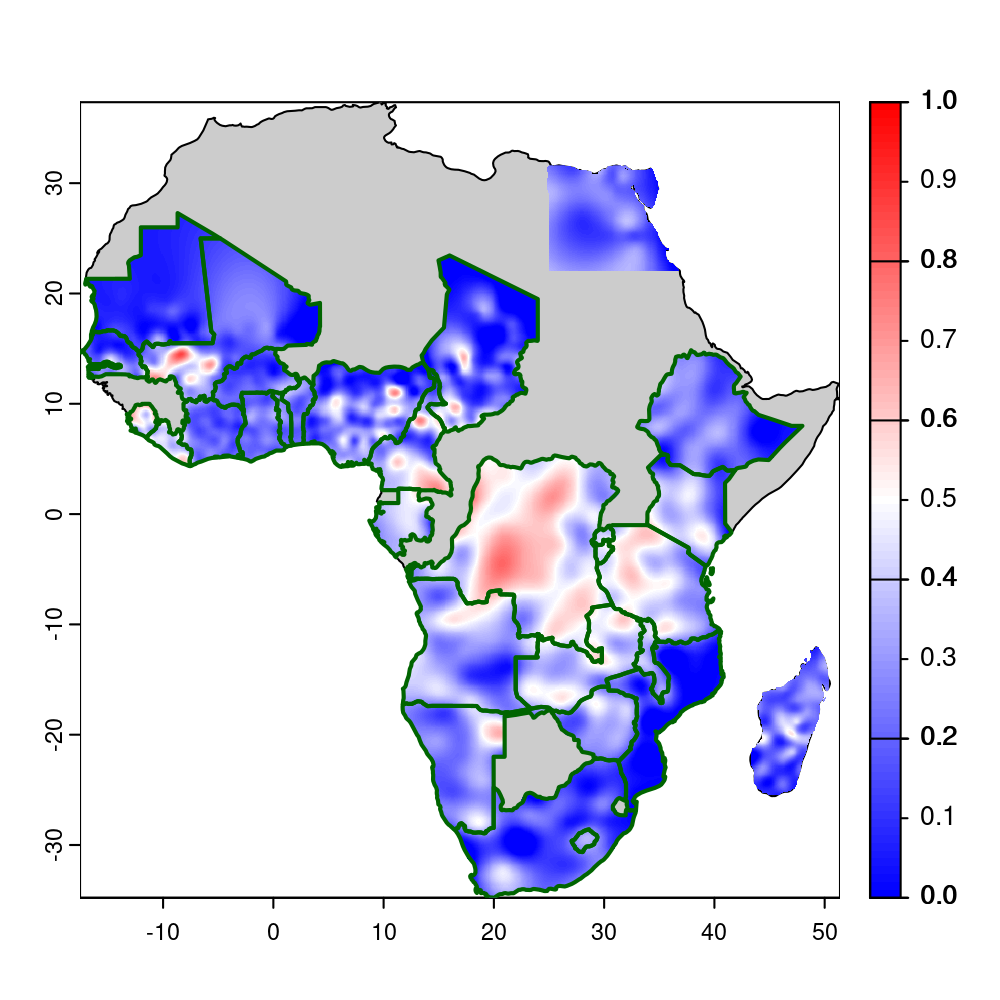
\includegraphics[trim=0cm 1cm 0cm 0cm, scale=0.55]{figure/africa-IPV-exposure-plot-1.png}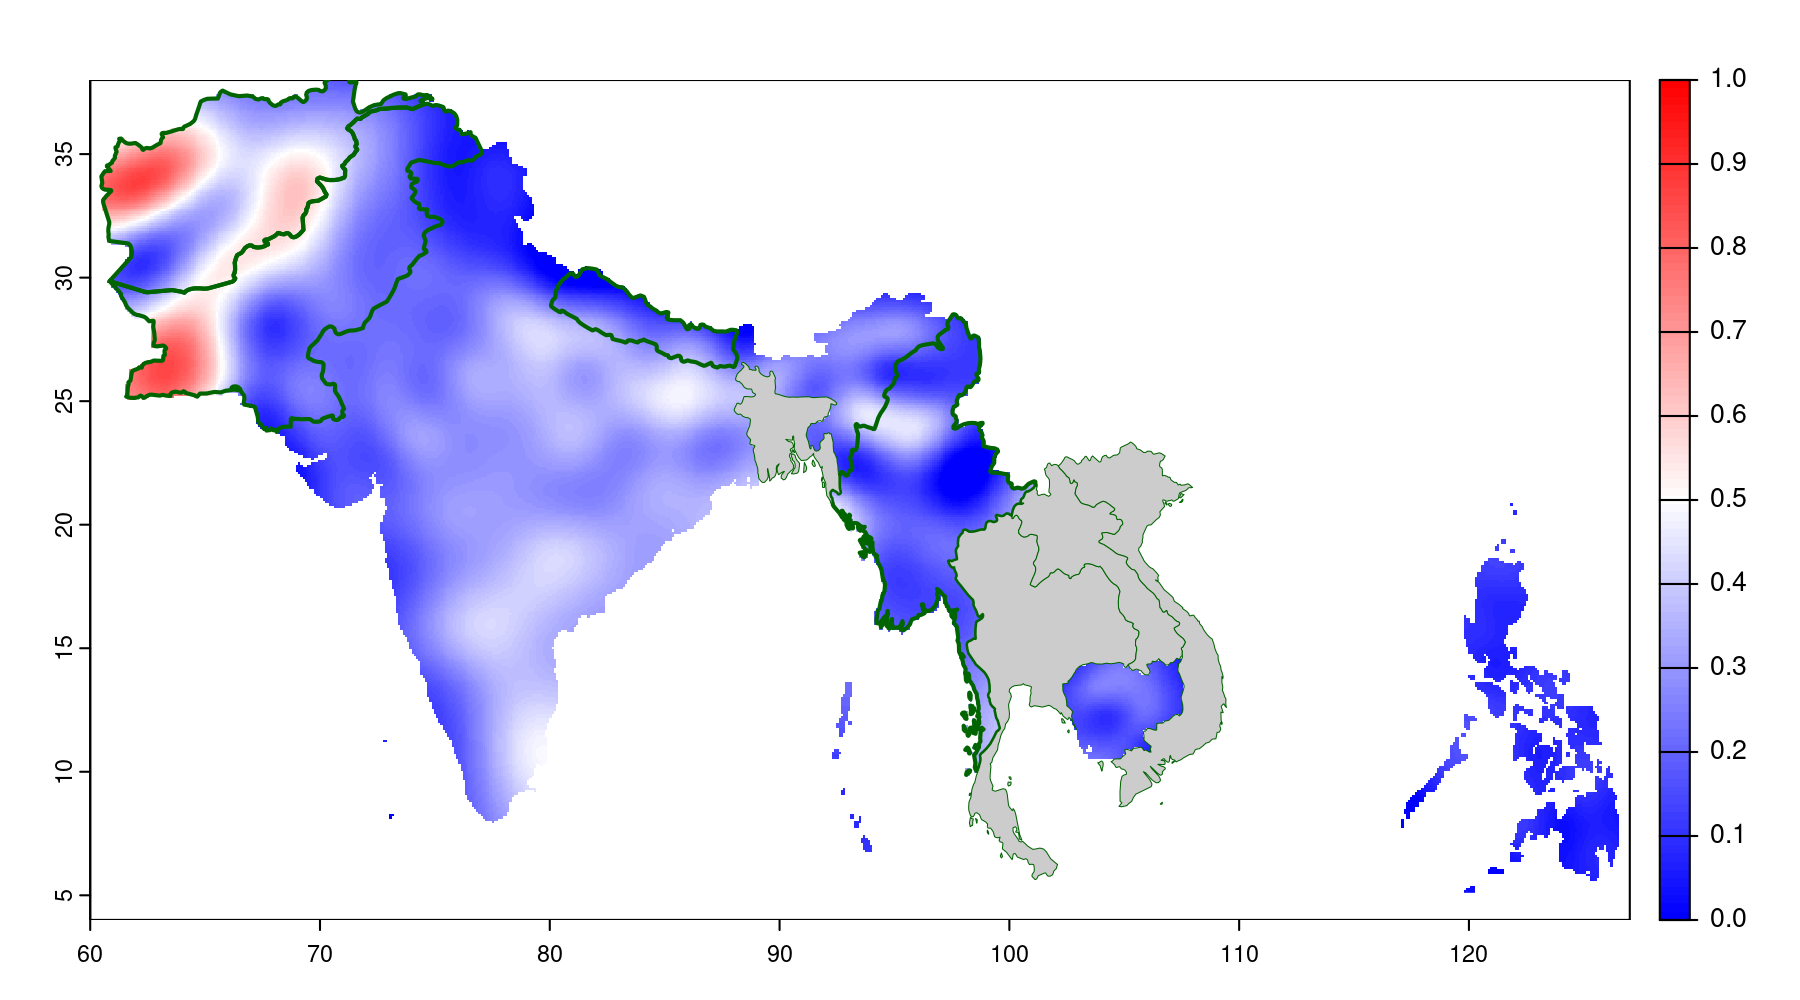
\includegraphics[trim=0cm 0.25cm 2cm 0cm, clip, scale=0.30]{figure/asia-IPV-exposure-1.png}
  \caption{Estimated proportion of wives who have experienced violence from their current husband. Left: Africa, n = 150173; number of sites = 19572, Right: South Asia: n = 156142; number of sites = 21473. Countries without data colored gray.}
\end{figure}

Figure 2 presents the estimated proportion of women in Africa and
South Asia who believe that intimate partner violence (IPV) can be
justified. The regions with the highest levels of IPV acceptance tend
to overlap with those reporting the highest levels of IPV
exposure—such as Afghanistan, Pakistan, and the Democratic Republic of
the Congo.

Notably, across both continents, the belief that IPV can be justified
is often more widespread than reported personal exposure to IPV. In
many regions with comparatively low reported exposure, more than 50
percent of women still believe that IPV can be justified. This pattern
is evident in countries such as Senegal, Mali, Chad, Ethiopia, Kenya,
southeastern India, Myanmar, and Cambodia.

As with exposure, country borders generally do not coincide with stark
shifts in attitudes toward IPV; neighboring regions across borders
often display similar levels of acceptance.

\begin{figure}
  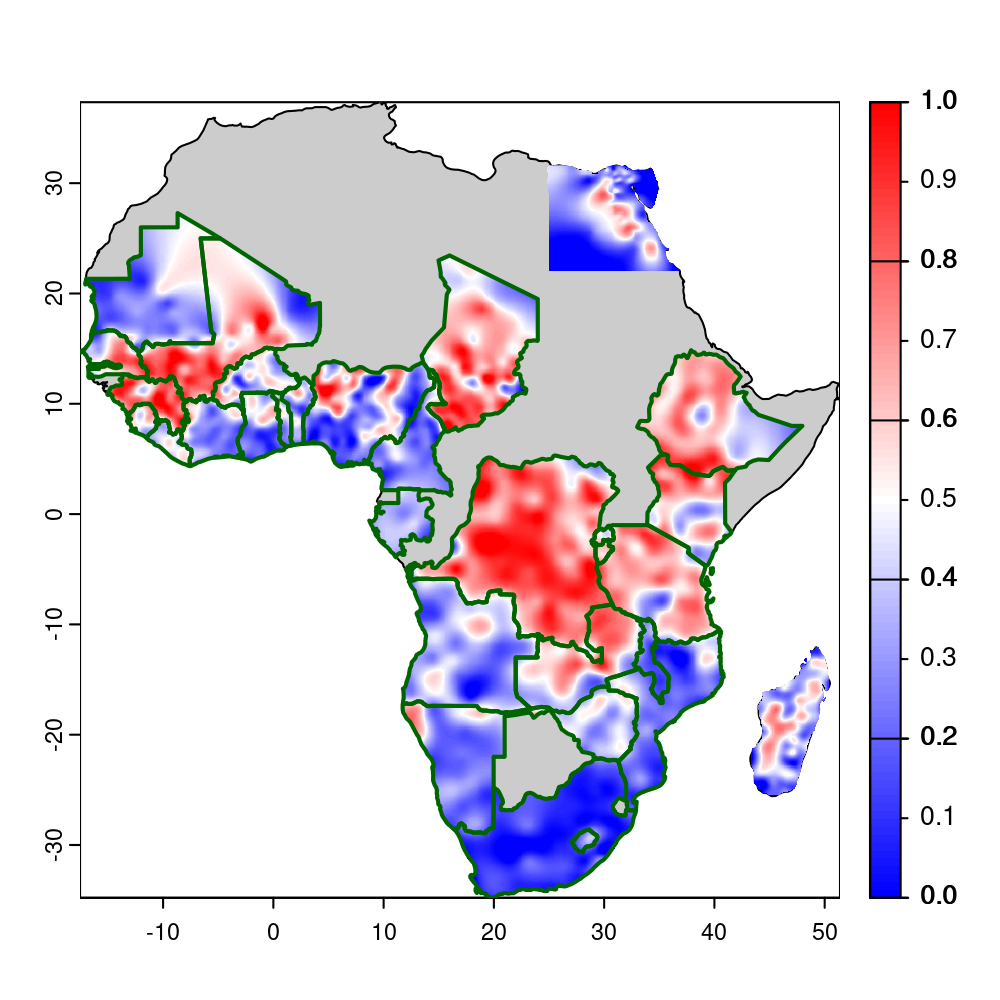
\includegraphics[trim=0cm 1cm 0cm 0cm, scale=0.55]{figure/africa-IPV-attitudes-plot-1.png}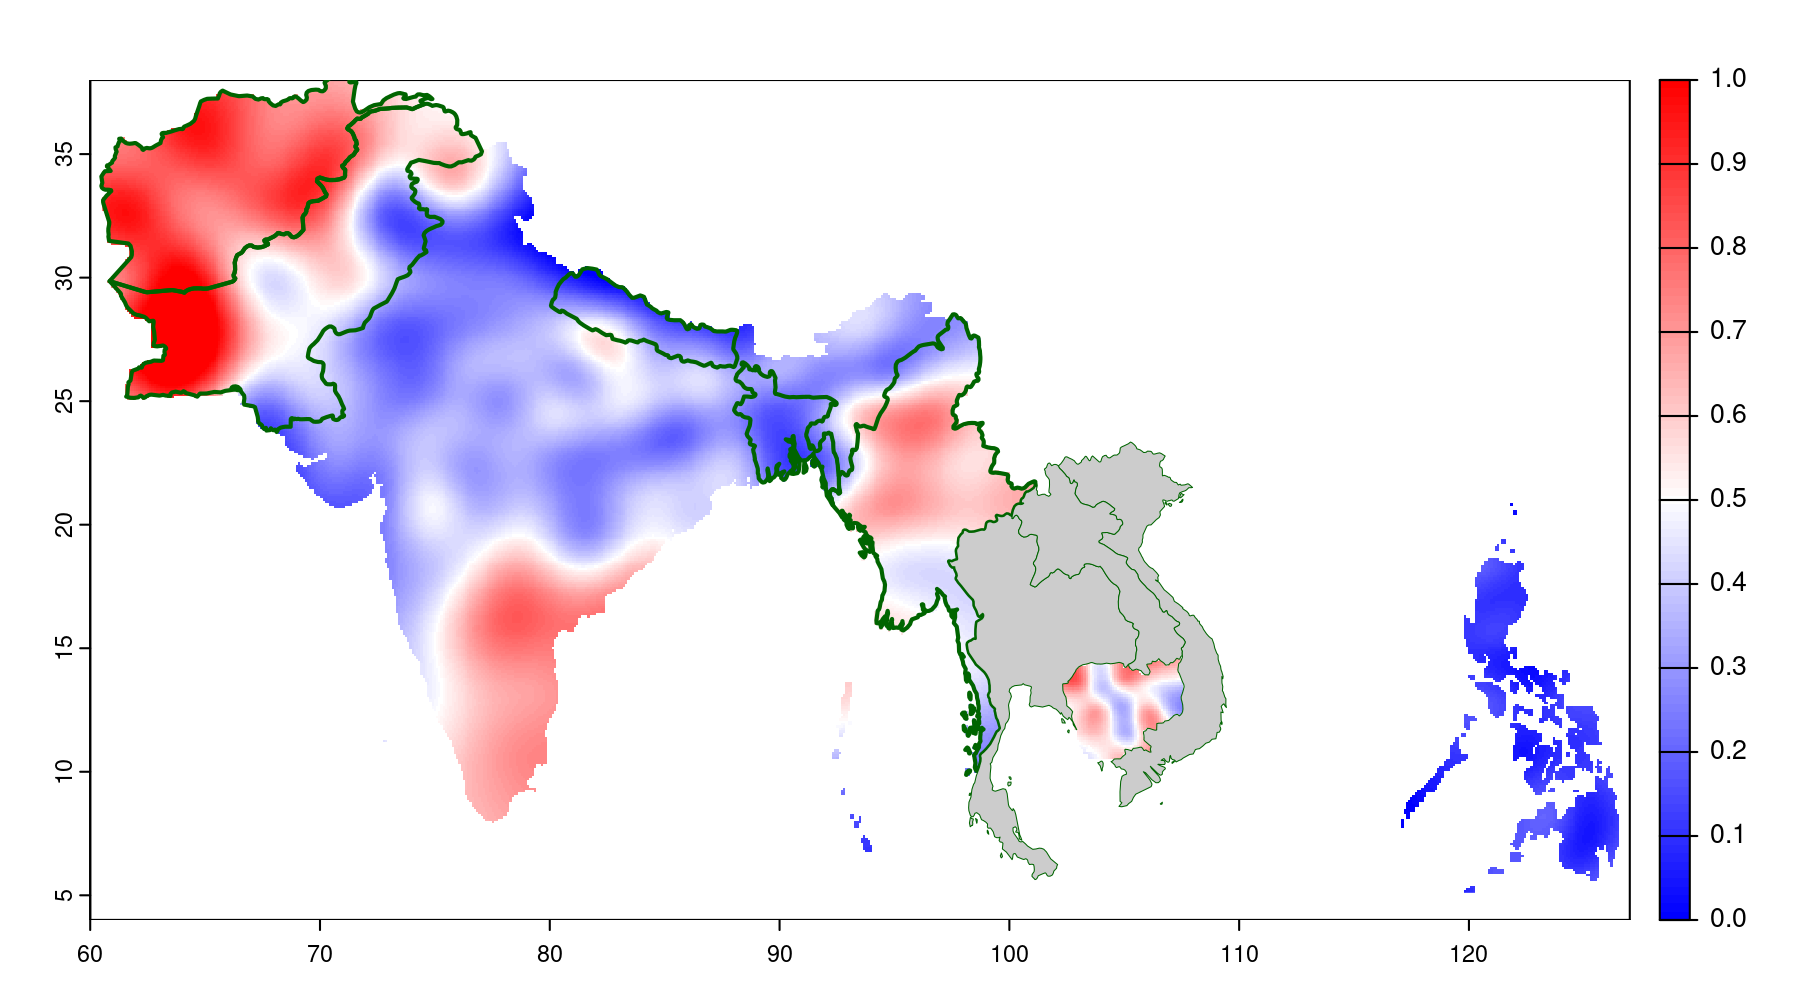
\includegraphics[trim=0cm 0.25cm 2cm 0cm, clip, scale=0.30]{figure/asia-IPV-attitudes-plot-1.png}
  \caption{Estimated proportion of women who thinks wife beating can be justified. Left: Africa, n = 461180; number of sites = 20248. Right: South Asia. n = 334042; number of sites = 22166. Countries without data colored gray.}
\end{figure}

Among men, 27 per cent justify IPV, and in most countries, there are
significantly more women than men who justify IPV. As mentioned above,
this result is in line with previous research (Speizer, 2010; Uthman,
Lawoko, et al., 2009). We will not dwell into the issue to why women are
more prone to accept men's violence against women than the men are, but
we will shed light on the association between differences between men
and women's attitudes to IPV and women's risk of experience IPV.

\subsection{Testing of hypotheses}
This section is based on the three different regression models
described in the methods section. Table 2 and Figure 3 are based on
the base model and are relevant for the two hypotheses, while Figure 4
and 5 is based on model 2 and 3 respectively and used to evaluate the
interaction effects.

The first column with estimates in Table 3 shows the bivariate odd-ratio
(OR) estimates for all our independent variables. These ORs are of
limited interest but give a starting point against which our base model
can be interpreted. They also show that all our independent variables
initially behave as expected. The last two rows in columns 2 and 3 show
the variance of the random intercepts derived from an empty model, i.e.,
a model without any independent variables. As illustrated by Figure 1,
the variance between countries is substantial and there is also a
considerable variance between neighbourhoods within countries.

\begin{longtable}[]{@{}
  >{\raggedright\arraybackslash}p{0.45\linewidth}
  >{\raggedright\arraybackslash}p{0.13\linewidth}
  >{\raggedright\arraybackslash}p{0.08\linewidth}
  >{\raggedright\arraybackslash}p{0.13\linewidth}
  >{\raggedright\arraybackslash}p{0.13\linewidth}@{}}  
\toprule
  & \multicolumn{2}{l}{Bivariate estimates} & \multicolumn{2}{l}{Base model estimates} \\
\midrule
\endhead
& Odds ratio & \emph{P\textgreater z} & Odds ratio &
\emph{P\textgreater z} \\
  Intercept & & & 0.47 & \emph{0.171} \\
  & & & & \\
\emph{Spouses' justifications of IPV} & & & & \\
Only Wife accept IPV & 2.07 & \emph{0.000} & 1.90 & \emph{0.000} \\
Only Husband accept IPV & 1.44 & \emph{0.000} & 1.32 & \emph{0.000} \\
Wife \& husband accept IPV & 3.18 & \emph{0.000} & 2.43 &
\emph{0.000} \\
& & & & \\
% \emph{N-JustIPV} & & & & \\
  Neighbourhood justifications IPV & 3.58 & \emph{0.000} & 1.72 &
\emph{0.000} \\
GDI: Gender Equality Index & 0.40 & \emph{0.011} & 0.28 &
\emph{0.073} \\
& & & & \\
\emph{Spouses' decision on health} & & & & \\
Wife decides & 1.52 & \emph{0.004} & 1.52 & \emph{0.000} \\
Husband decides & 1.46 & \emph{0.003} & 1.09 & \emph{0.077} \\
Spouses don't agree & 1.30 & \emph{0.000} & 1.16 & \emph{0.000} \\
& & & & \\
\emph{Spouses' decisions on purchases} & & & & \\
Wife decides & 1.56 & \emph{0.000} & 1.46 & \emph{0.000} \\
Husband decides & 1.54 & \emph{0.002} & 1.25 & \emph{0.000} \\
Spouses don't agree & 1.37 & \emph{0.000} & 1.19 & \emph{0.000} \\
& & & & \\
\emph{Wife's education} & & & & \\
incomplete primary & 0.87 & \emph{0.280} & 1.06 & \emph{0.102} \\
complete primary & 0.86 & \emph{0.176} & 1.04 & \emph{0.450} \\
incomplete secondary & 0.67 & \emph{0.000} & 0.94 & \emph{0.296} \\
complete secondary & 0.51 & \emph{0.000} & 0.78 & \emph{0.039} \\
higher & 0.36 & \emph{0.000} & 0.58 & \emph{0.000} \\
& & & & \\
\emph{Difference in spouses' education} & & & & \\
Wife has higher education & .93 & \emph{0.263} & 1.04 & \emph{0.091} \\
Husband has higher education & 1.10 & \emph{0.001} & 0.96 &
\emph{0.034} \\
& & & & \\
\emph{Spouses' literacy} & & & & \\
Wife illiterate & 1.60 & \emph{0.000} & 1.08 & \emph{0.105} \\
Husband illiterate & 1.36 & \emph{0.000} & 1.09 & \emph{0.004} \\
Both spouses' illiterate & 1.79 & \emph{0.000} & 1.11 & \emph{0.023} \\
& & & & \\
IWI & 0.28 & \emph{0.000} & 0.59 & \emph{0.000} \\
Wife's age (ln) & 1.15 & \emph{0.045} & 0.90 & \emph{0.092} \\
Number of Children (ln) & 1.45 & \emph{0.000} & 1.26 & \emph{0.000} \\
GDP per capita & 0.38 & \emph{0.006} & 0.88 & \emph{0.794} \\
& & & & \\
& Variance & Std & Variance & Std \\
Random intercept: Country & 1.98 & \emph{0.446} & 0.37 & \emph{0.069} \\
Random intercept: Neighbourhood & 0.74 & \emph{0.098} & 0.80 &
\emph{0.092} \\
  \bottomrule
  \caption{Odds Ratio estimates with 95\% confidence intervals from the base model.}
\end{longtable}

Looking at the base model estimates for the term relevant the first
hypothesis, ``Women living in a neighbourhood where IPV is widely
accepted suffer from an increased IPV risk.'', the coefficient for the
term ``Neighbourhood justifications IPV'' is 1.72 which means that the
odds for being exposed to IPV is 1.72 times higher in neighbourhoods
where all women thinks IPV can be justified than in neighbourhoods
where no woman holds that view. The left-hand side of figure 3
visualises the effect size in terms of probabilities rather than odds
ratio.\footnote{In order to be able to predict probabilities we had to
  set the other variables in the model to some value, and here we set
  them to their mean values.} In the range of neighbourhood
justification levels visualised in figure 3, about 0.1 to a bit over
0.8, the predicted probability of IPV increases from just below 0.2 to
about 0.28. Hence, there is a clear neighbourhood effect that operates
independently of individual justification of IPV, and hypothesis 1 has
thus found empirical support.

\begin{figure}
  \centering
  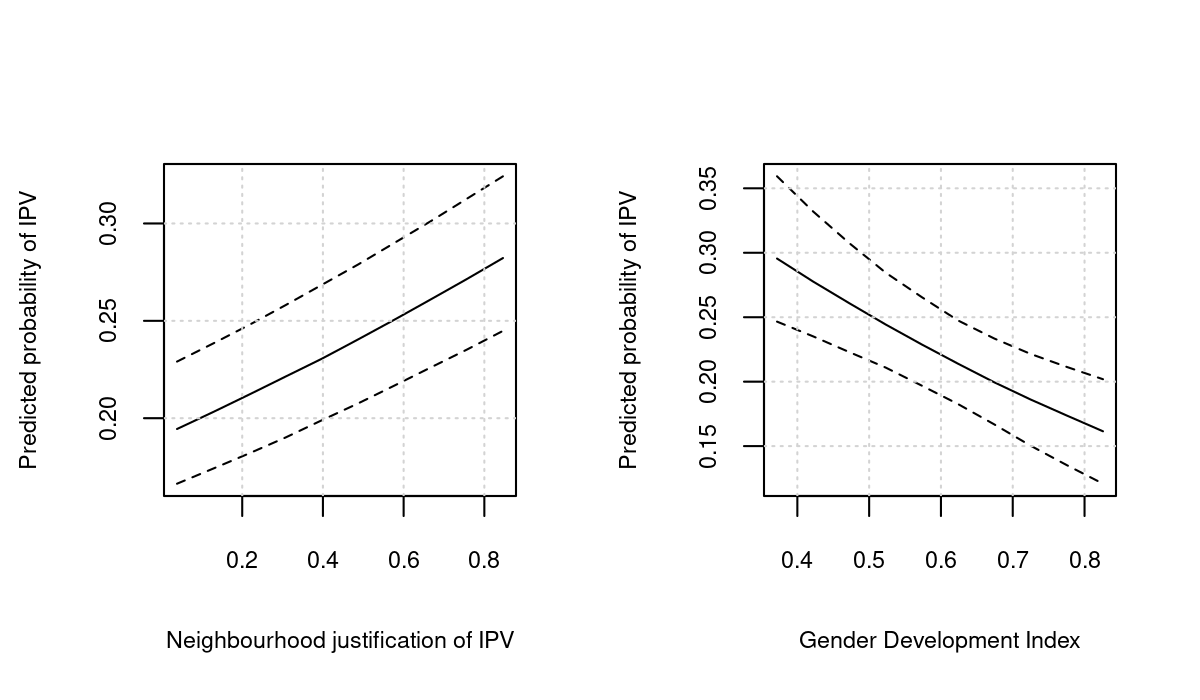
\includegraphics[scale = 0.75]{figure/base-model-plot-1}
  \caption{Left: Predicted probabilities of IPV for typical values of Neighbourhood justification of IPV. Right: Predicted probabilities of IPV for the typical values of the Gender Development Index. Typical values defined as the values above the 10th percentile and below the 90th percentile. Predictions based on the base model. Credible intervals based on 95\% of the sampled parameters.}
\end{figure}

As for the second hypothesis, ``Net of spouse's and neighbours'
justification of IPV, the IPV risk is lower in countries that are more
gender equal.'', the coefficient for the relevant term ``GDI: Gender
Equality Index'' is 0.28, suggesting that it is 3-4 times more common
to be exposed IPV in countries with the highest GDI in the sample than
in countries with lowest GDI in the sample. In figure 3, the right
hand side plot, we have graphed the predicted probability of IPV for
the rather conservative range of GDI values (the 10th percentiles in
both ends of the range are excluded), and in that range the predicted
probability of IPV drops from 0.3 to a bit above 0.15. To conclude:
even under control for attitudes toward IPV both in the individual
level and the neigbourhood level, gender equality at the country level
has a substantial effect, and higher levels of gender equality
decreases IPV.

Regarding the control variables, we can see that lack of cooperation
in decision-making increases the wife-IPV risk. Secondary and higher
education decrease the risk, while spouses' illiteracy increases it.
The risk is lower in more wealthy households and higher in households
with many children.

\subsection{Testing of interactions}

%% Comments are my original text, without comments is revised with
%% help of ChatGPT.

% Interaction 1 concerns a possible moderation of the effect of the
% attitudes of the neighbouring women's attitudes to IPV on the
% individual woman's risk of being exposed to IPV. Specifically, we
% explore if the attitude toward IPV of the couple appears to moderate
% this neighbourhood effect. To be clear, the probability for a couple
% to have a certain attitude is not generally independent on the levels
% of IPV justification in the neighbourhood, if you know that 0 percent
% of the women in the neighbourhood thinks IPV can be justfied, we can
% not find a couple where the woman thinks IPV can be justified.
% However, when we calculate the attitude of ``neighbourhood'', we do
% that separately for each individual woman, which means that two women
% in the same village will have different values on that variable if
% they do not share the same attitude. This way, it is perfectly
% possible for a women to be one of the categories: ``Only wife
% justifies IPV'', ``Both justify IPV'' and in a neighbourhood where 0
% percent of the (other) women thinks IPV can be justifed.

% rom the confirmation of hypothesis 1 we know that even under control
% for the attitudes in the couple, living in a neighbourhood where a
% large percent of women thinks IPV can be justified increases the
% likelihood of beeing exposed to IPV. The question now is are all four
% types of couples as sensitive in this regard, or are some types of
% couple more sensitive to the attitudes of the neighbouring women?

% To test this we use model 2 and the results are visualised in figure
% 4.

% \begin{figure}
%   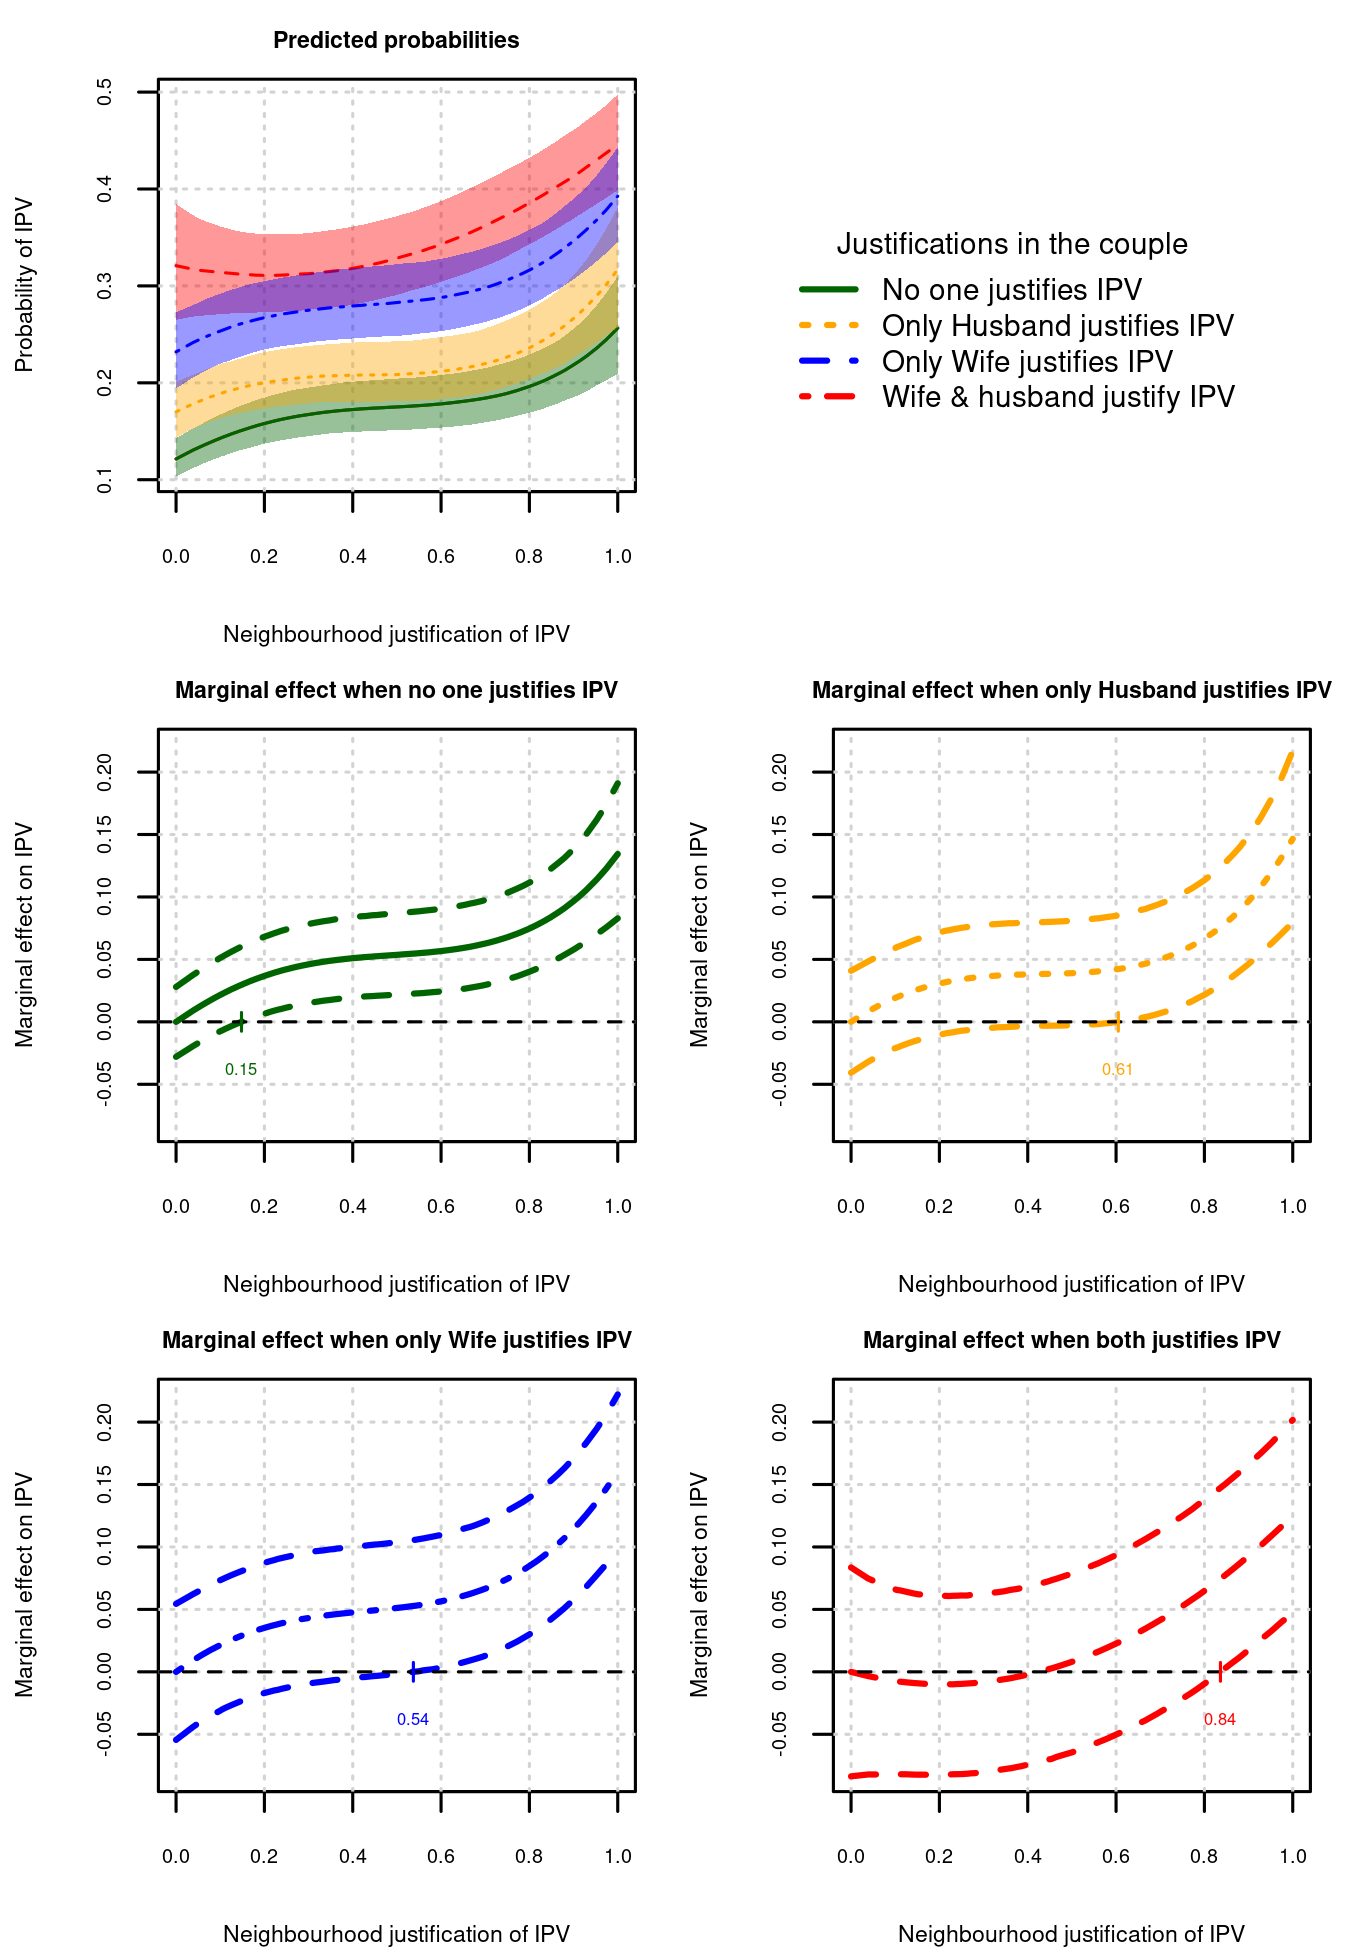
\includegraphics{figure/dual-plot-1.png}
%   \caption{Predicted probabilities and Marginal effects for a woman to be
% exposed to IPV conditioned on the attitudes of the other women in the local
% area in different types of couples. Credible intervals corresponding to
% 95\% of the parameter samples. n = 148393.}
% \end{figure}

% Contrary to our expectations, the type of couple that turned out to
% be most sensitive to the attitudes toward IPV of the neighbourhood is
% the couple were no one thinks IPV can be justified. The difference in
% predicted probability between such couples living and neighbourhoods
% where no other woman thinks IPV can be justified and neighbourhoods
% where all women thinks IPV can be justified is about 0.14. The
% credible intervals of the marginal effect of neighbourhood
% justification of IPV overlaps zero only until the proportion of women
% in the neighbourhood becomes 0.15. Putting these number into
% perspective we can compare with the couples where both wife and
% husband thinks IPV can be justified, the marginal effect is
% essentially zero at least until the level of neighbouring women who
% thinks IPV can be justified increases above 0.5, the lower bound of
% the credible interval exceed zero only when 84\% of the neighbouring
% women thinks IPV can be justified.

% In neighbourhoods were all or almost other women thinks IPV can be
% justified, the marginal effect is essentially the same in all types of
% couples, the differences, and thus the interaction effect, lie in the
% neighbourhood types were this is less common.

% More importantly, having a neighbourhood where very few women thinks
% IPV can be justified can be said to have a protective effect, but it
% is not the norm of the majority that appears to be most important
% here. Instead, what matters most is if at least one third of all women
% in the neighbourhood rejects IPV.

Interaction 1 examines whether the neighbourhood norm regarding IPV
justification moderates an individual woman’s risk of experiencing IPV
and, in particular, whether this neighbourhood effect varies by the
couple’s own attitudes.

Because a couple's stance on IPV is naturally correlated with the
prevailing neighbourhood norm (e.g., no couple can justify IPV if 0\%
of local women do), we compute the “neighbourhood justification”
variable separately for each woman. In other words, a woman’s own
response is excluded from the neighbourhood proportion; two women in the
same village who give different answers therefore receive different
neighbourhood justification scores. This construction allows, for example, a wife
who alone thinks IPV can be justified in an otherwise IPV rejecting
village to belong to the “only wife justifies IPV” category while
still having a neighbourhood justification score of zero.

Consistent with Hypothesis 1, living among more women who justify IPV
raises the probability of experiencing IPV, even after controlling for
the couple’s own attitudes. The crucial question is whether all four
couple-types are equally sensitive to the neighbourhood climate.

\begin{figure}
  \label{fig:interaction1}
  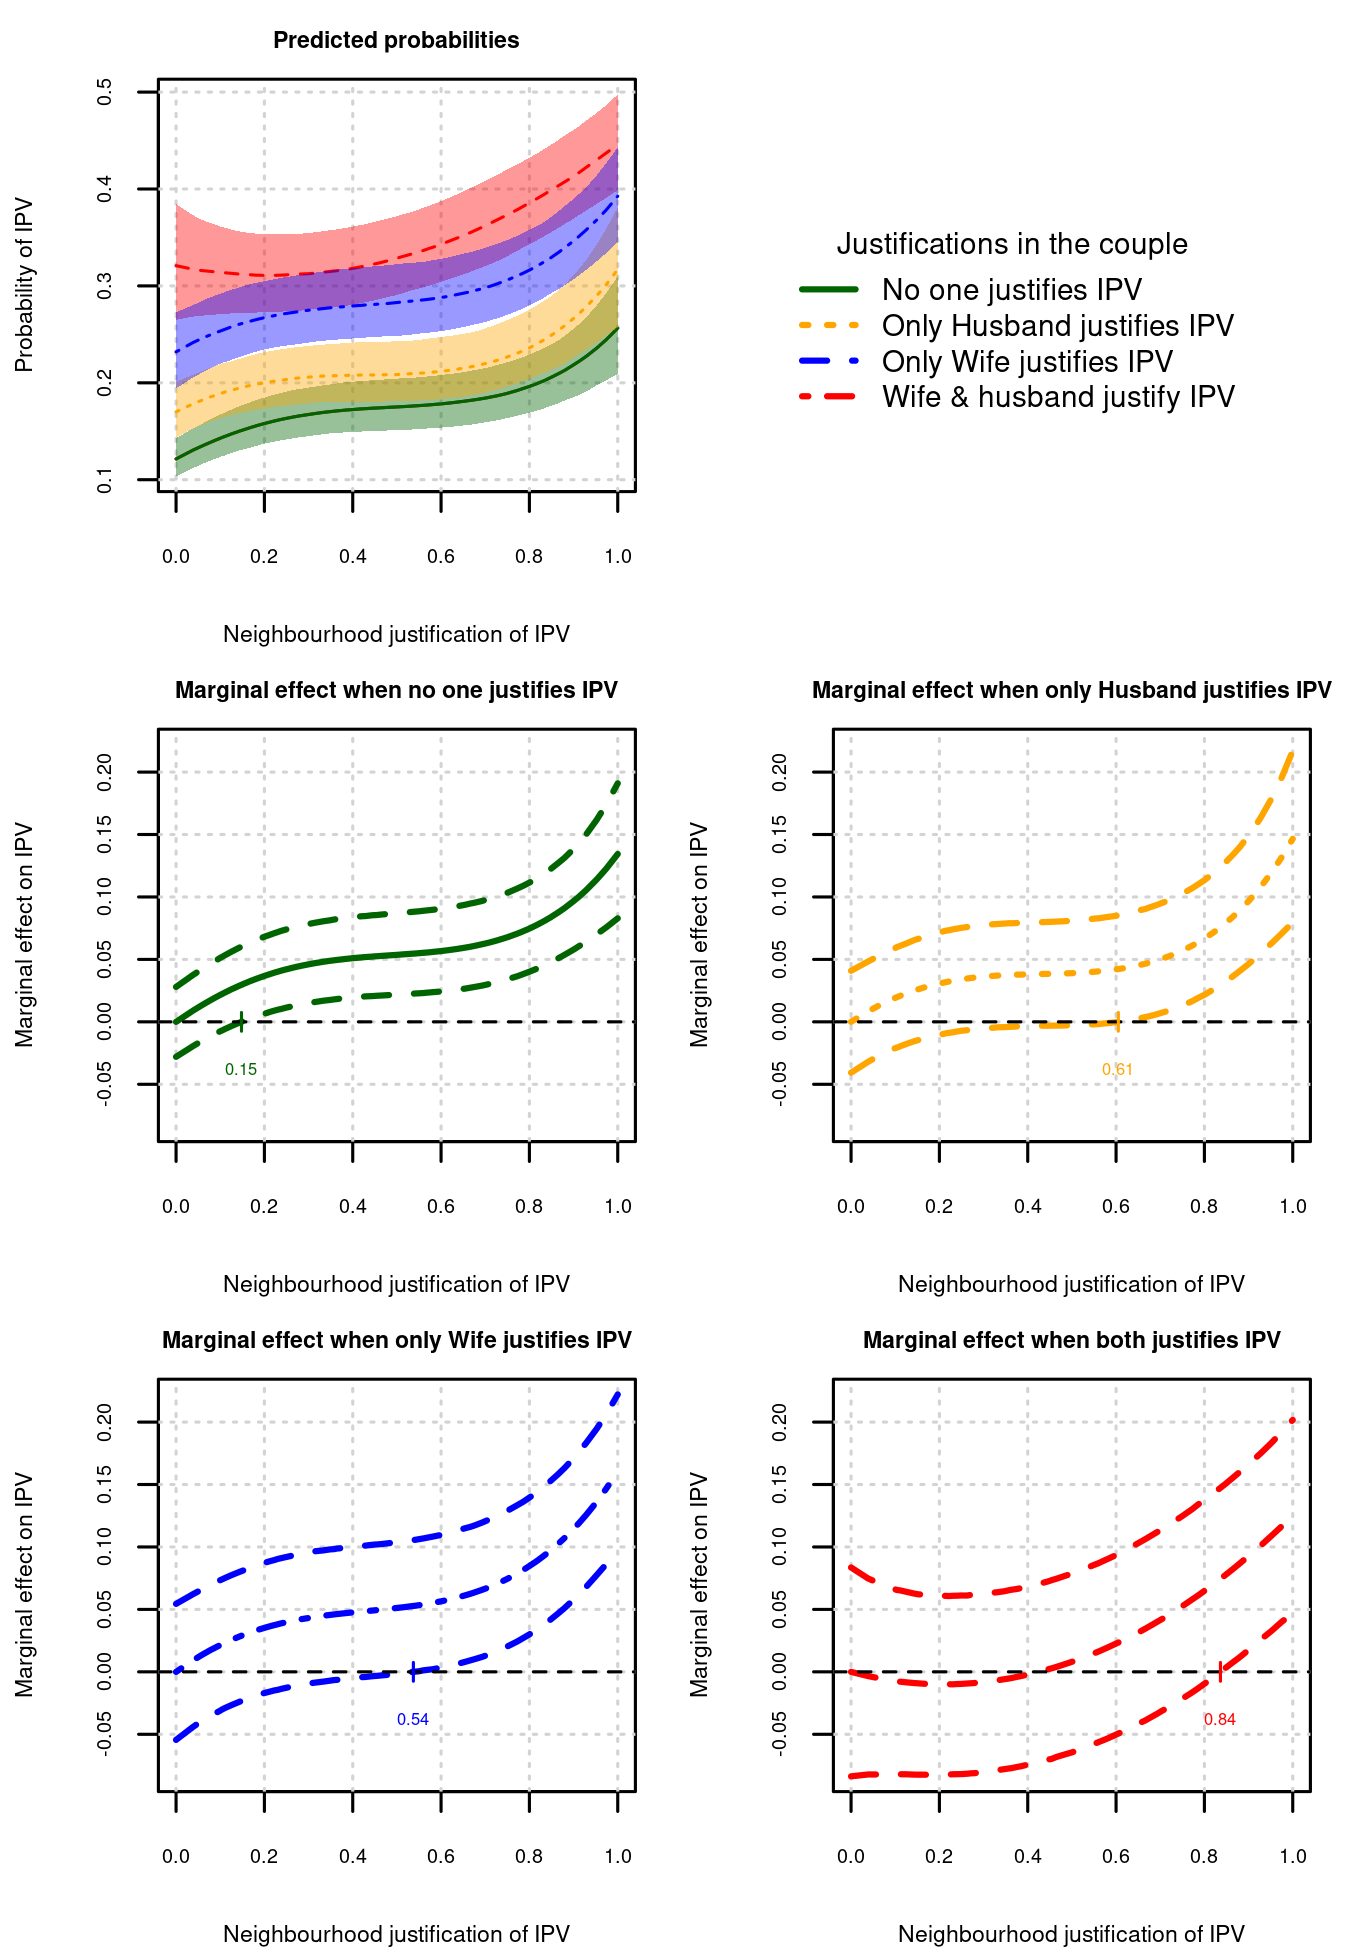
\includegraphics{figure/dual-plot-1.png}
  \caption{Predicted probabilities and Marginal effects for a woman to be
exposed to IPV conditioned on the attitudes of the other women in the local
area in different types of couples. Credible intervals corresponding to
95\% of the parameter samples. n = 148393.}
\end{figure}

Contrary to our expectation, the couple type most sensitive to
neighbourhood norms is the one in which \emph{neither} partner
believes IPV can be justified. For such couples, predicted IPV risk
rises by roughly 0.14 when moving from a neighbourhood in which no
other woman justifies IPV to one in which all do. The 95\% credible
interval for this marginal effect exceeds zero once the share of
justifying women in the neighbourhood surpasses about 15\%.

By contrast, when \emph{both} partners believe IPV can be justified,
the marginal effect of the neighbourhood norm is essentially nil until
the local proportion of justifying women exceeds 50\%. The lower bound
of the credible interval does not clear zero until that proportion
reaches roughly 84\%.

At the extreme—neighbourhoods where nearly every woman thinks IPV can
be justified—the marginal effect converges across couple types; the
interaction arises mainly in settings where IPV justification is
uncommon or only moderately prevalent.

A neighbourhood in which very few women justify IPV appears to afford
a protective effect, but the critical threshold is not full consensus.
Instead, the sharpest decline in IPV risk occurs once roughly
one-third of women in the neighbourhood reject IPV, regardless of the
attitudes in the individual couple.

% \subsubsection{The interaction of the attitudes in the couple and the Gender Equality
%   in the country}

% First follows my original text, then a version based on suggestions
% from ChatGPT

% In figure \vref{fig:interaction2} we show the visualise
% the results from model 3, this contains an interaction effect
% between the country level variable Gender Equality Index (GDI) and
% the attitudes of the individual couples. This model is restricted to
% be linear in logit, so even if its non-linear in probability it is
% by definition
% \href{https://en.wikipedia.org/wiki/Monotonic_function}{strictly monotonic}.\footnote{This
% make model 3 different from model 2 which, in the bottom right plot
% of figure \vref{fig:interaction1}, displayed a local minimum at
% Neighbourhood justification of IPV at around 0.2.}

% \begin{figure}
%   \label{fig:interaction2}
%   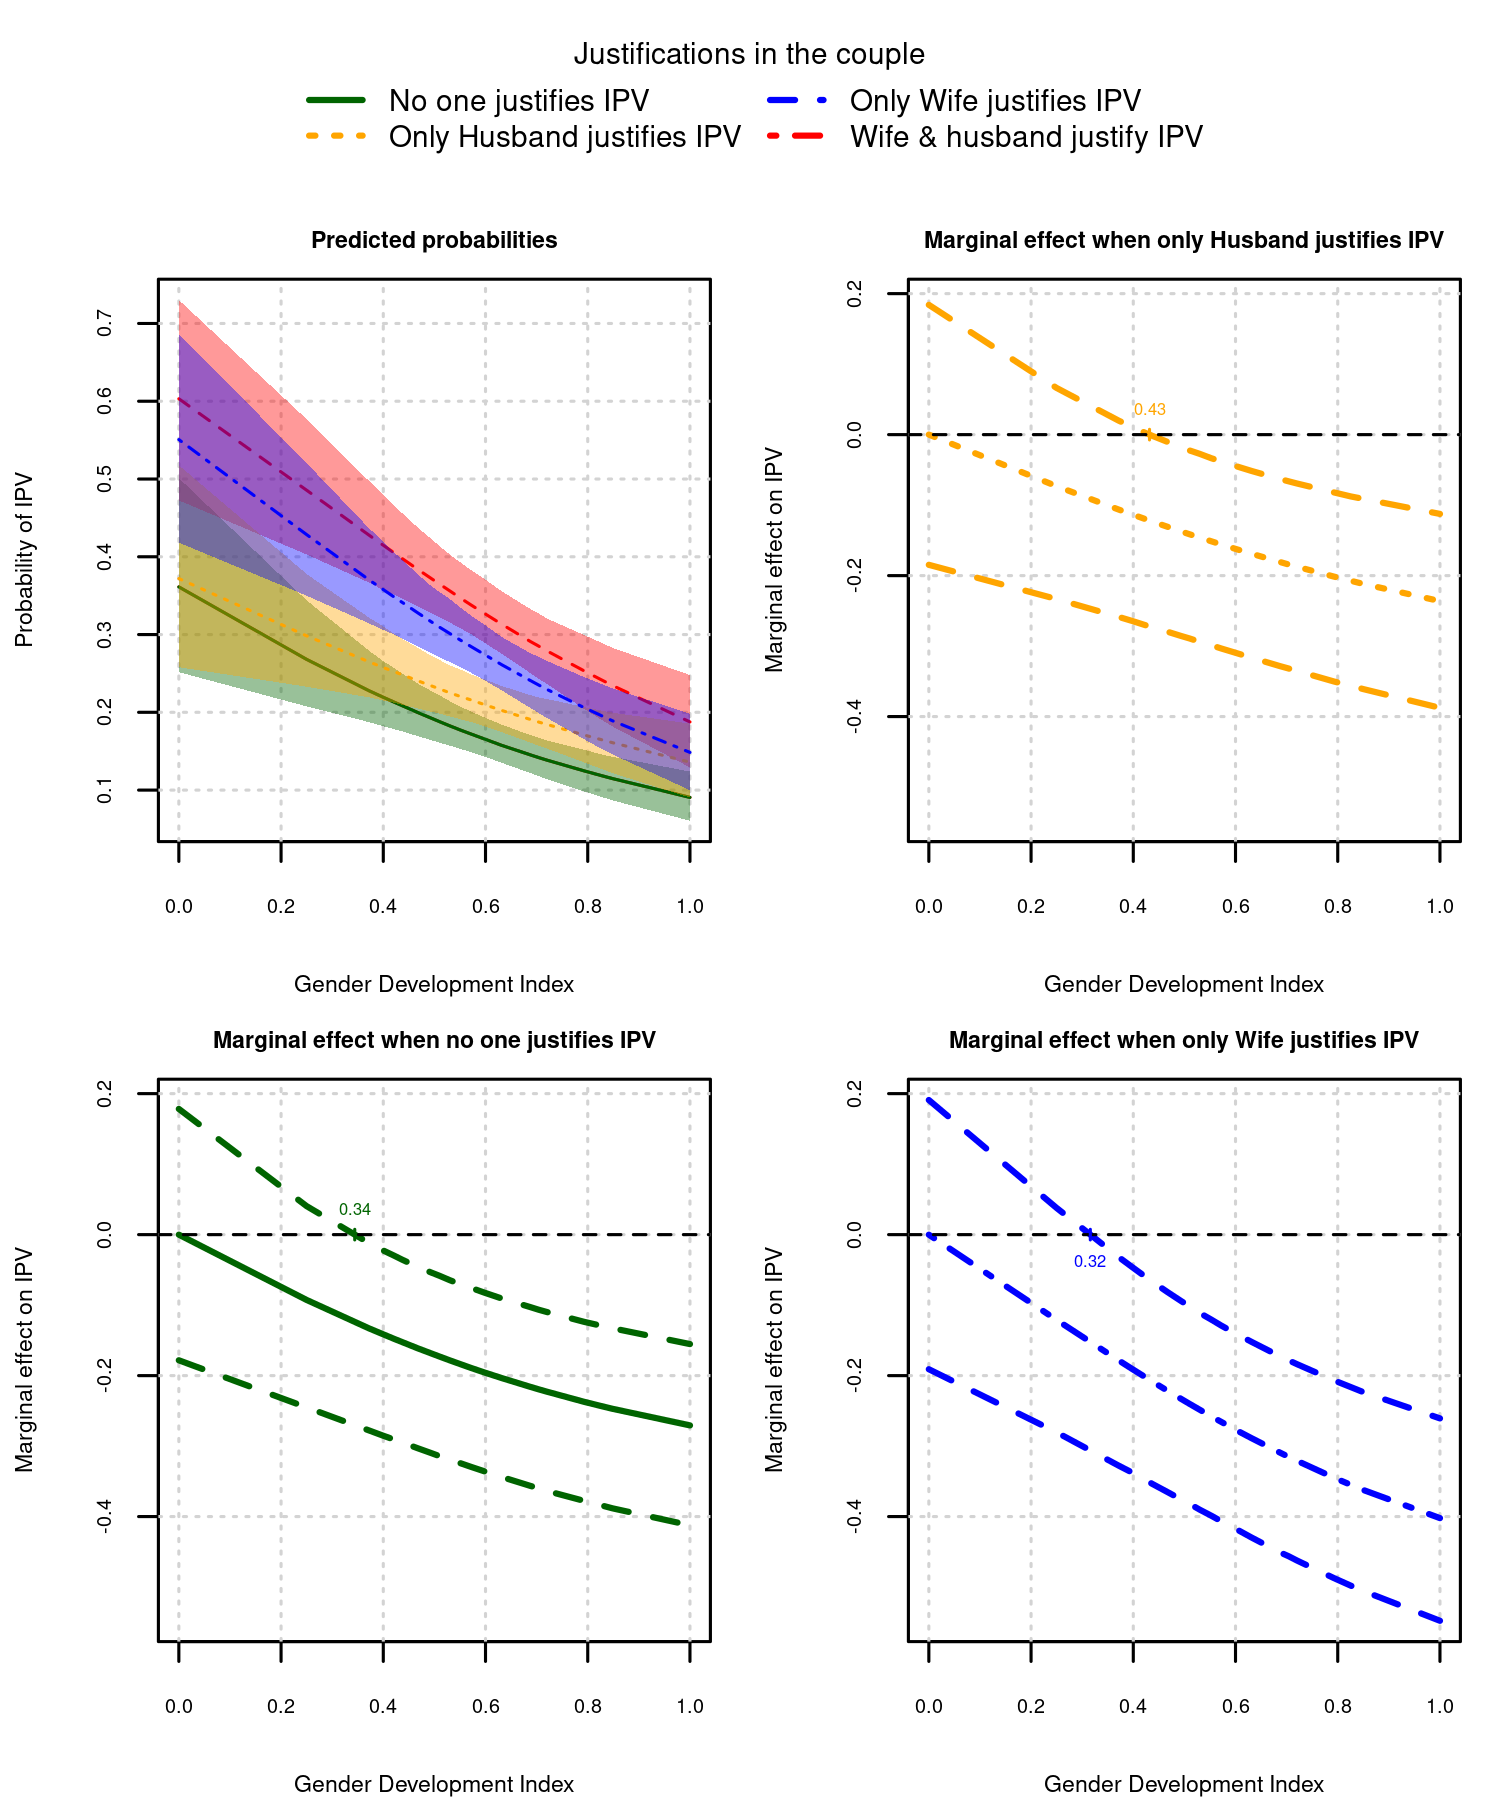
\includegraphics{figure/take-2-1.png}
%   \caption{Predicted probabilities for a woman to be exposed to IPV
%     conditioned on the Gender Development Index (top lef) and the
%     Marginal effect of the Gender Development Index on the probability
%     of IPV in different types of couples. Credible intervals
%     corresponding to 95\% of the parameter samples. n = 148421}
% \end{figure}

% Looking at the graph with predicted probabilities of IPV, the general
% pattern is that the higher the GDI, the lower the
% probability of IPV, regardless of the attitudes in the couple. There
% are some subtle differences but overall the curves for different types
% of couples are similar, in particular ``Wife \& Husband justify IPV''
% and ``Only Wife justifes IPV'' are so similar that we only graphed the
% marginal effect of the latter.

% The graphs with the marginal effects of GDI show that the protective
% effect of GDI is highest when ``Only Wife justifies IPV'',
% \footnote{The marginal effect of GDI when both wife and husband
%   justifies IPV (not shown) is almost the same as for couples where
%   ``Only Wife justifies IPV''} slightly lower for couples where ``No
% one justifies IPV'' and smallest when ``Only Husband justifies IPV''.
% The graphed marginal effects are all statistically signficantly
% different from each other, but their striking visual simularities
% makes it hard to draw any other conclusions than GDI decreases the
% probability of IPV generally, and in similar ways for all types of
% couples, so that in countries with low GDI the differences in risk of
% IPV in couples with different attitudes are larger than in countries
% with high GDI.

%% End of revised text

\subsubsection{Interaction between Couple Attitudes and National Gender Development}

Figure \vref{fig:interaction2} visualises the results from model 3,
which includes an interaction between the country-level
Gender Development Index (GDI) and the couple’s own attitudes
toward IPV.\footnote{Because the model is linear in the logit, the
predicted probabilities are, by construction, a
\href{https://en.wikipedia.org/wiki/Monotonic_function}{strictly monotonic}
function of the GDI within each attitude category.  In contrast,
model~2 (bottom-right panel of Figure~\vref{fig:interaction1}) allowed
a local minimum at a neighbourhood-justification level of roughly
0.2.}

\begin{figure}
  \centering
  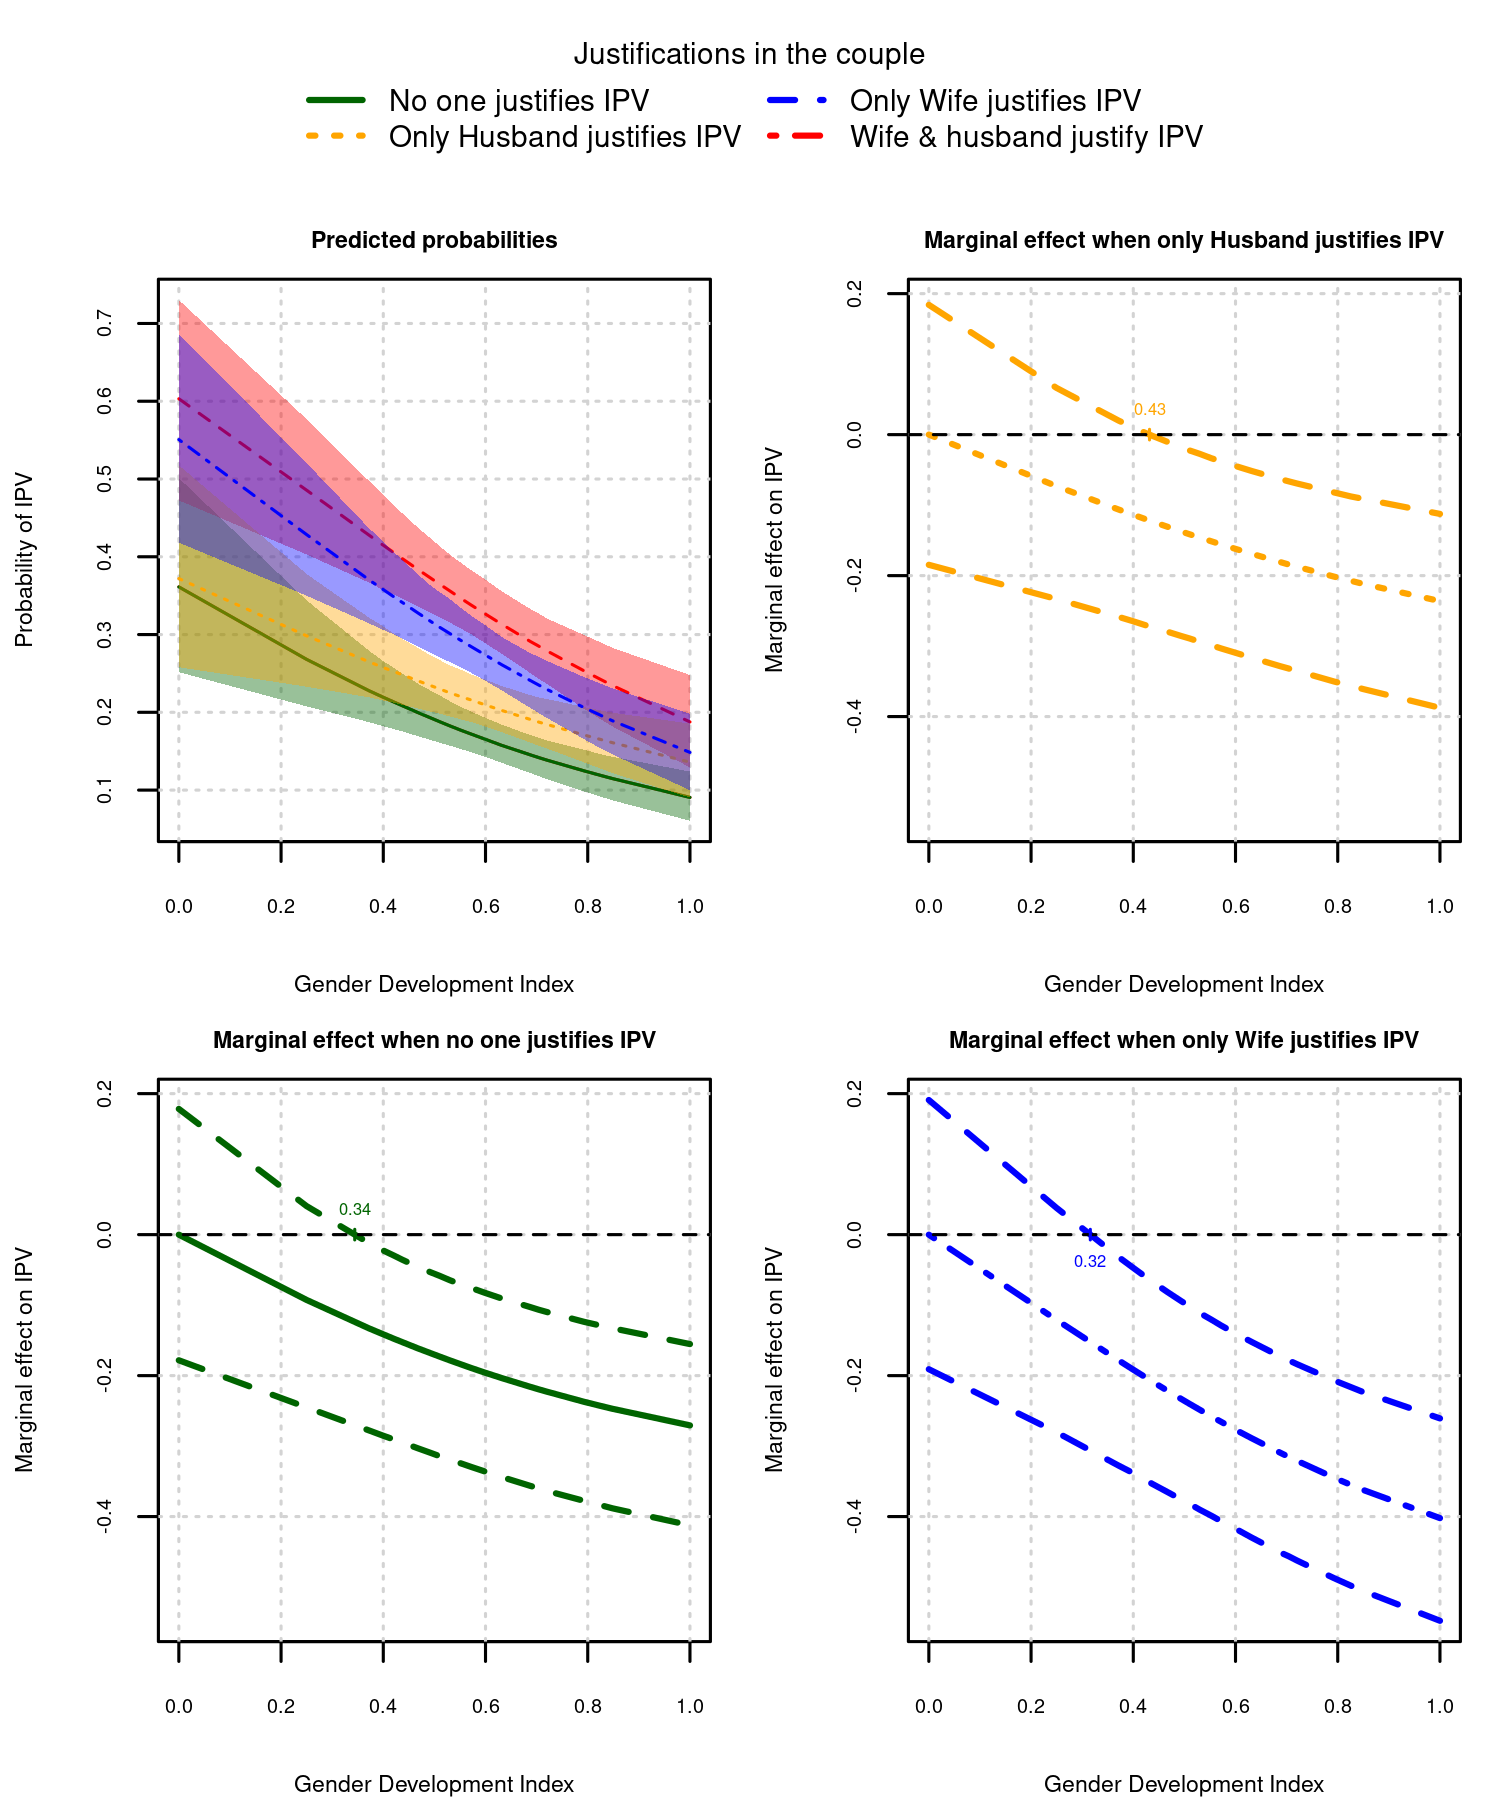
\includegraphics{figure/take-2-1.png}
  \caption{Predicted probabilities that a woman experiences IPV
    (top-left) and the marginal effect of the Gender Development Index
    on that probability for different couple-attitude categories.
    Shaded areas show 95\% credible intervals; $n = 148{,}421$.}
  \label{fig:interaction2}
\end{figure}

Across all four couple types, a higher GDI is associated with a lower
predicted probability of IPV. The two categories in which the wife
believes IPV can be justified—\emph{only wife justifies} and
\emph{both justify}—display almost identical curves, so we plot the
marginal effect only for the former to avoid redundancy.

The protective effect of GDI (i.e., the slope in the marginal-effect
panels) is strongest when \emph{only the wife} justifies IPV, slightly
weaker when \emph{neither partner} does, and weakest when
\emph{only the husband} does.\footnote{The unplotted curve for
  \emph{both justify} is virtually indistinguishable from the \emph{only wife}
  curve.} Although the 95 \% credible intervals of the regression
coefficients indicate that these slopes differ statistically, their
visual similarity suggests a common substantive conclusion: improving
national gender development reduces IPV risk across all couple types.
%% End of revised text

\section{Conclusions}
Our multi-level analysis of 294,583 couples from 36 low- and
middle-income countries and 32 Indian states yields a clear message:
\emph{where a woman lives matters at least as much as whether she or
  her husband thinks IPV can be justified or not}.

Local communities where violence is widely viewed as justifiable place
all women at heightened risk of IPV, regardless of the convictions in
the individual couple. The proportion of women who reject IPV
regardless of circumstances does not need to be in majority to have a
protective influence, instead our analyses show that most of the
protective effect of informal social control is reached once \emph{one
  third of the neighbouring women unconditionally rejects IPV}. To get
even stronger protection from informal social control the proportion
of neighbouring women who rejects IPV needs to get above 80\%.

Unfortunately, it is evident from the maps we provide that in large
parts of Africa and South Asia this is not the situation.

%% Original text
% When comparing women's risk of IPV between countries, we found that
% gender equality in health, education and wealth at the country level is
% associated with decreased risk of IPV. This pattern hold across all
% couple-attitude categories, indicating that structural gender equality
% provides a societal buffer even the husband, the wife, or both of them
% think IPV can be justified.

%% ChatGPT revised version

Cross-national comparisons show that greater gender equality in
health, education, and income—as captured by the Gender Development
Index—reduces IPV risk across the board. Crucially, this protective
effect holds even when the wife, the husband, or both believe IPV can
be justified, indicating that structural gender equality provides a
societal buffer against violence in the home.

Taken together, the findings imply that interventions aimed solely at
changing individual attitudes or partner dynamics will be insufficient
unless they are reinforced by efforts that (i) shift community norms
toward zero tolerance of wife-beating and (ii) advance women’s
structural position in education, health, and economic life.

\section{Limitations}
Because this is an observational study based on cross-sectional data,
we cannot draw empirically derived causal conclusions; what we observe
are associations. Self-reported IPV is likely under-stated where
stigma remains high.

Additionally, the data do not allow us to determine the
timing between events. We know if the mother has been exposed to IPV,
and we know if any or both spouses justify IPV, but we do not know the
order in which these events occurred. At the same time, as argued above,
we do not expect unidirectional causation to be found. The relationship
between occurrence, attitudes towards IPV, and empowerment of women is
most probably best understood in terms of good and evil circles. Even
though we estimated fixed effects for both the country and sampling
cluster, we cannot rule out the possibility that we missed individual or
household-related confounders. Data on IPV are collected from a DHS
subsample, and there is a risk of selection bias. In particular that
women who are most exposed to IPV and men that often execute IPV might
be more likely to decline to participate in this specific module. Hence,
there is a risk that we underestimate both the prevalence of IPV and the
association between IPV and attitudes.

Selection into the domestic-violence module may bias levels downward,
although such bias would need to covary systematically with both
contextual measures to overturn our main associations.

\section{Discussion}
That women are suffering from intimate person violence (IPV) is global
human rights problem. Our results point to the importance of social
embeddedness, personal beliefs and the link between beliefs and action
do not exist in a social vacuum. Even after including individual
attitudes towards IPV, individual IPV risk is higher in neighbourhoods
where a large share of neighbouring women accepts IPV. This is in line
with theories of stigmatization. In a social setting where IPV is
condemned, the risk of stigma has a restraining effect independently
of individual beliefs.

In line with previous research (Uthman, Lawoko, et al., 2009), we found
that acceptance of IPV is less common among men. We also find that when
only the husband accepts IPV, the wife's risk of being exposed to IPV is
lower compared to when only the wife accepts IPV. Our interpretation is
that when women are empowered to reject the use of IPV, men are less
likely to execute IPV even though they believe they have the right to do
so.

SOME MORE REFLEXIONS ON WHAT MAKES THIS STUDY STAND OUT AND HOW IT
RELATES TO PREVIOUS RESEARCH SHOULD MAKE FOR A NICE FINISH.

\section{References}
Arefaynie, M., Bitew, G., Amsalu, E. T., Kefale, B., Muche, A., Fentaw,
Z., Dewau, R., Melaku, M. S., Yalew, M., Adane, B., Adane, M., Chanie,
M. G., Ayele, W. M., \& Damtie, Y. (2021). Determinants of wife-beating
acceptance among reproductive age women in Ethiopia: a multilevel
analysis of 2016 Ethiopian demographic and health survey {[}Article{]}.
\emph{Bmc Womens Health}, \emph{21}(1), 10, Article 342.
\url{https://doi.org/10.1186/s12905-021-01484-1}

Bates, D., Mächler, M., Bolker, B. M., \& Walker, S. C. (2015). Fitting
Linear Mixed-Effects Models Using lme4. \emph{Journal of Statistical
Software}, \emph{67}(1), 1-48.
\url{https://doi.org/10.18637/jss.v067.i01}

Beyer, K., Wallis, A. B., \& Hamberger, L. K. (2015). Neighborhood
Environment and Intimate Partner Violence: A Systematic Review
{[}Article{]}. \emph{Trauma Violence \& Abuse}, \emph{16}(1), 16-47.
\url{https://doi.org/10.1177/1524838013515758}

Carlson, G. J., Kordas, K., \& Murray-Kolb, L. E. (2015). Associations
between women's autonomy and child nutritional status: a review of the
literature {[}Review{]}. \emph{Maternal and Child Nutrition},
\emph{11}(4), 452-482. \url{https://doi.org/10.1111/mcn.12113}

Chowdhury, S. R., \& Mathur, K. (2021). Why Do Women Support
Wife-Beating More Than Men in India? Evidence From the National Family
Health Survey (2015-2016) {[}Article; Early Access{]}. \emph{Family
Journal}, 10, Article 10664807211022000.
\url{https://doi.org/10.1177/10664807211022000}

Coleman, J. (1988). Social capital in the creation of human capital.
\emph{American Journal of Sociology}, \emph{94}(Suppl), 95-120.

Cunningham, K., Ruel, M., Ferguson, E., \& Uauy, R. (2015). Women's
empowerment and child nutritional status in South Asia: a synthesis of
the literature {[}Review{]}. \emph{Maternal and Child Nutrition},
\emph{11}(1), 1-19. \url{https://doi.org/10.1111/mcn.12125}

Devries, K. M., Mak, J. Y., Garcia-Moreno, C., Petzold, M., Child, J.
C., Falder, G., Lim, S., Bacchus, L. J., Engell, R. E., \& Rosenfeld, L.
(2013). The global prevalence of intimate partner violence against
women. \emph{Science}, \emph{340}(6140), 1527-1528.

Eckstein, J. J. (2011). Reasons for Staying in Intimately Violent
Relationships: Comparisons of Men and Women and Messages Communicated to
Self and Others. \emph{Journal of Family Violence}, \emph{26}(1), 21-30.
\url{https://doi.org/10.1007/s10896-010-9338-0}

Elvin-Nowak, Y. M. S., Backman-Enelius, M. M., Jonas, W. C., Eriksson,
J. A., Ahlund, D. S., \& Barimani, M. M. (2023). Intimate partner
violence and negative health consequences: A cross-sectional study among
women in a regional sample in Sweden {[}Article{]}. \emph{Scandinavian
Journal of Public Health}, \emph{51}(4), 636-643.
\url{https://doi.org/10.1177/14034948221148056}

Eze-Ajoku, E., Fakeye, O., Atanda, A., \& Sosina, O. A. (2022). Economic
Empowerment and Tolerance of Domestic Violence Among Married Women: A
Cross-Sectional Study {[}Article{]}. \emph{Journal of Interpersonal
Violence}, \emph{37}(5-6), NP2719-NP2746, Article 0886260520943727.
\url{https://doi.org/10.1177/0886260520943727}

Flood, M., \& Pease, B. (2009). FACTORS INFLUENCING ATTITUDES TO
VIOLENCE AGAINST WOMEN {[}Review{]}. \emph{Trauma Violence \& Abuse},
\emph{10}(2), 125-142. \url{https://doi.org/10.1177/1524838009334131}

Global\_Data\_Lab. (2024). \emph{Sub-national GDI}. Retrieved November 6
from \url{https://globaldatalab.org/shdi/metadata/sgdi/}

Goffman, E. (2009). \emph{Stigma: Notes on the management of spoiled
identity}. Simon and schuster.

Haque, M. A., Choudhury, N., Ahmed, S. M. T., Farzana, F. D., Ali, M.,
Rahman, S. S., Faruque, A. S. G., Raihan, M. H., \& Ahmed, T. (2022).
Factors Associated with Domestic Violence in Rural Bangladesh
{[}Article{]}. \emph{Journal of Interpersonal Violence}, \emph{37}(3-4),
1248-1269, Article 0886260520922353.
\url{https://doi.org/10.1177/0886260520922353}

Heaton, T. B., \& Forste, R. (2008). Domestic violence, couple
interaction and children's health in Latin America {[}Article{]}.
\emph{Journal of Family Violence}, \emph{23}(3), 183-193.
\url{https://doi.org/10.1007/s10896-007-9142-7}

Krause, K. H., Gordon-Roberts, R., VanderEnde, K., Schuler, S. R., \&
Yount, K. M. (2016). Why Do Women Justify Violence Against Wives More
Often Than Do Men in Vietnam? {[}Article{]}. \emph{Journal of
Interpersonal Violence}, \emph{31}(19), 3150-3173.
\url{https://doi.org/10.1177/0886260515584343}

Lelaurain, S., Fonte, D., Giger, J. C., Guignard, S., \& Lo Monaco, G.
(2021). Legitimizing Intimate Partner Violence: The Role of Romantic
Love and the Mediating Effect of Patriarchal Ideologies {[}Article{]}.
\emph{Journal of Interpersonal Violence}, \emph{36}(13-14), 6351-6368.
\url{https://doi.org/10.1177/0886260518818427}

Luke, N., Schuler, S. R., Mai, B. T. T., Thien, P. V., \& Minh, T. H.
(2007). Exploring couple attributes and attitudes and marital violence
in Vietnam {[}Article{]}. \emph{Violence against Women}, \emph{13}(1),
5-27. \url{https://doi.org/10.1177/1077801206295112}

Machio, P. M., Kimani, D. N., Kariuki, P. C., Ng'ang'a, A. M., \&
Njoroge, M. M. (2022). Social Capital and Women's Empowerment
{[}Article; Early Access{]}. \emph{Forum for Social Economics}, 19.
\url{https://doi.org/10.1080/07360932.2022.2115526}

Mookerjee, M., Ojha, M., \& Roy, S. (2022). Who's your Neighbour? Social
Influences on Domestic Violence {[}Article{]}. \emph{Journal of
Development Studies}, \emph{58}(2), 350-369.
\url{https://doi.org/10.1080/00220388.2021.1969012}

Park, Y., Song, J. Y., Kim, Y. O., Paik, S., \& Sullivan, K. (2024).
Interpersonal Violence in Five Regions in Asia: Ecological Risk Factors
Associated with Perceptions of Justifiability of Violence {[}; Early
Access{]}. \emph{Journal of Interpersonal Violence}, 33.
\url{https://doi.org/10.1177/08862605241271418}

Patil, V. P., \& Khanna, S. (2022). Trends in attitudinal acceptance of
wife-beating, domestic violence, and help-seeking among married women in
Nepal {[}Article; Early Access{]}. \emph{Journal of Biosocial Science},
16, Article Pii s0021932022000165.
\url{https://doi.org/10.1017/s0021932022000165}

Pinchevsky, G. M., \& Wright, E. M. (2012). The Impact of Neighborhoods
on Intimate Partner Violence and Victimization {[}Article{]}.
\emph{Trauma Violence \& Abuse}, \emph{13}(2), 112-132.
\url{https://doi.org/10.1177/1524838012445641}

Pratley, P. (2016). Associations between quantitative measures of
women's empowerment and access to care and health status for mothers and
their children: A systematic review of evidence from the developing
world {[}Review{]}. \emph{Social Science \& Medicine}, \emph{169},
119-131. \url{https://doi.org/10.1016/j.socscimed.2016.08.001}

Rawlings, S., \& Siddique, Z. (2020). Domestic Violence and Child
Mortality in the Developing World {[}Article{]}. \emph{Oxford Bulletin
of Economics and Statistics}, \emph{82}(4), 723-750.
\url{https://doi.org/10.1111/obes.12357}

Sado, L., Spaho, A., \& Hotchkiss, D. R. (2014). The influence of
women's empowerment on maternal health care utilization: Evidence from
Albania {[}Article{]}. \emph{Social Science \& Medicine}, \emph{114},
169-177. \url{https://doi.org/10.1016/j.socscimed.2014.05.047}

Sampson, R. J., Morenoff, J. D., \& Gannon-Rowley, T. (2002). Assessing
"neighborhood effects": Social processes and new directions in research
{[}Article{]}. \emph{Annual Review of Sociology}, \emph{28}, 443-478.
\url{https://doi.org/10.1146/annurev.soc.28.110601.141114}

Sardinha, L., Maheu-Giroux, M., Stockl, H., Meyer, S. R., \&
Garcia-Moreno, C. (2022). Global, regional, and national prevalence
estimates of physical or sexual, or both, intimate partner violence
against women in 2018 {[}Article{]}. \emph{Lancet}, \emph{399}(10327),
803-813. \url{https://doi.org/10.1016/s0140-6736(21)02664-7}

Schrubbe, L., Garcia-Moreno, C., Sardinha, L., \& Stockl, H. (2023).
Intimate partner violence against women during pregnancy: a systematic
review and meta-analysis protocol for producing global and regional
estimates {[}Review{]}. \emph{Systematic Reviews}, \emph{12}(1), 7,
Article 107. \url{https://doi.org/10.1186/s13643-023-02232-2}

Singh, B. P., Singh, K. K., \& Singh, N. (2014). Couple Interaction and
Predicting Vulnerability to Domestic Violence in Uttar Pradesh, India
{[}Article{]}. \emph{Journal of Interpersonal Violence}, \emph{29}(12),
2304-2324. \url{https://doi.org/10.1177/0886260513518432}

Smits, J., \& Steendijk, R. (2015). The International Wealth Index
(IWI). \emph{Social Indicators Research}, \emph{122}(1), 65-85.
\url{https://doi.org/10.1007/s11205-014-0683-x}

Speizer, I. S. (2010). Intimate Partner Violence Attitudes and
Experience Among Women and Men in Uganda. \emph{Journal of Interpersonal
Violence}, \emph{25}(7), 1224-1241.
\url{https://doi.org/10.1177/0886260509340550}

Stockl, H., Devries, K., Rotstein, A., Abrahams, N., Campbell, J.,
Watts, C., \& Moreno, C. G. (2013). The global prevalence of intimate
partner homicide: a systematic review {[}Review{]}. \emph{Lancet},
\emph{382}(9895), 859-865.
\url{https://doi.org/10.1016/s0140-6736(13)61030-2}

Uthman, O. A., Lawoko, S., \& Moradi, T. (2009). Factors associated with
attitudes towards intimate partner violence against women: a comparative
analysis of 17 sub-Saharan countries {[}Article{]}. \emph{Bmc
International Health and Human Rights}, \emph{9}, 15, Article 14.
\url{https://doi.org/10.1186/1472-698x-9-14}

Uthman, O. A., Moradi, T., \& Lawoko, S. (2009). The independent
contribution of individual-, neighbourhood-, and country-level
socioeconomic position on attitudes towards intimate partner violence
against women in sub-Saharan Africa: A multilevel model of direct and
moderating effects {[}Article{]}. \emph{Social Science \& Medicine},
\emph{68}(10), 1801-1809.
\url{https://doi.org/10.1016/j.socscimed.2009.02.045}

Wood, J. T. (2001). The normalization of violence in heterosexual
romantic relationships: Women's narratives of love and violence
{[}Article{]}. \emph{Journal of Social and Personal Relationships},
\emph{18}(2), 239-261. \url{https://doi.org/10.1177/0265407501182005}

\clearpage

\appendix

Table 1. Analytical variables derived from DHS.

\begin{longtable}[]{@{}
  >{\raggedright\arraybackslash}p{0.2\linewidth}
  >{\raggedright\arraybackslash}p{0.6\linewidth}
  >{\raggedright\arraybackslash}p{0.2\linewidth}@{}}  
\toprule
  Variable & Operationalization & DHS variables \\
\midrule
\endhead
& Main variables & \\
Wife experienced IPV (Wife-IPV) & Experienced any physical or sexual violence by intimate partner. & d106 d107 d108 \\
Spouses' justifying IPV (S-JustifyIPV) & 
\begin{minipage}[t]{\linewidth}\raggedright
IPV justified if wife: goes out without telling, neglect children,
argues with husband, refuses sex, or doesn't cook food properly?

\begin{enumerate}
\def\labelenumi{\arabic{enumi}.}
\item
  Nor wife, neither husband justify IPV.
\item
  Only wife justify IPV.
\item
  Only husband justify IPV.
\item
  Both wife and husband justify IPV.
\end{enumerate}
\end{minipage} & v/mv744a

v/mv744b

v/mv744c

v/mv744e \\
Neighbouring women justifying IPV (Neigh-JustifyIPV) & Proportion of women in the DHS sampling cluster that Justify IPV & V743a v743b v743d \\
GDI & Subnational Gender development index. Normalized to 0 -- 1 & GDL data \\
& Control variables & \\
Spouse deciding on healthcare (S-DecideH) and purchases (S-DecideP) & 
\begin{minipage}[t]{\linewidth}\raggedright
Decide on wife's healthcare and decide on large household purchases:

\begin{enumerate}
\def\labelenumi{\arabic{enumi}.}
\item
  Husband and wife jointly decides.
\item
  Both agree that wife decides.
\item
  Both agree that husband decides.
\item
  Spouses do not agree.
\end{enumerate}

Comment: In a few cases wife decides together with another person in the
household. These cases have been coded as 1.
\end{minipage} & v/mv743a

v/mv743a \\
Wife's education (Wife-EDU) &
\begin{minipage}[t]{\linewidth}\raggedright
Wifes's education:

\begin{enumerate}
\def\labelenumi{\arabic{enumi}.}
\item
  No education.
\item
  Incomplete primary.
\item
  Primary.
\item
  Incomplete Secondary.
\item
  Secondary
\item
  Higher
\end{enumerate}
\end{minipage} & v149 \\
Differences in spouses' education (S-DiffEDU) &
\begin{minipage}[t]{\linewidth}\raggedright
Wife's education in relation to husband's education:

\begin{enumerate}
\def\labelenumi{\arabic{enumi}.}
\item
  No difference
\item
  Wife has higher education
\item
  Husband has higher education
\end{enumerate}
\end{minipage} & v/mv149 \\
International Wealth Index (IWI) & The households' possession of basic
assets. IWI normalized to 0 -- 1 & Derived from DHS using code from
GDL \\
Wife's age (Wife-AGE) & The natural logarithm of Wife's age when
interviewed & v012 \\
Number of children in the household (Num-Child) & The natural logarithm
of number of children in the household & bidx\_01 -20 \\
GDP per capita & Logarithm of Gross National Income per Capita.
Normalized to 0 -- 1 & GDL data \\
\bottomrule
\end{longtable}

Wives' exposure to IPV, wives and husbands' justification of
IPV by country, and GDI.

\begin{figure}
  \label{fig:splines-model-2}
  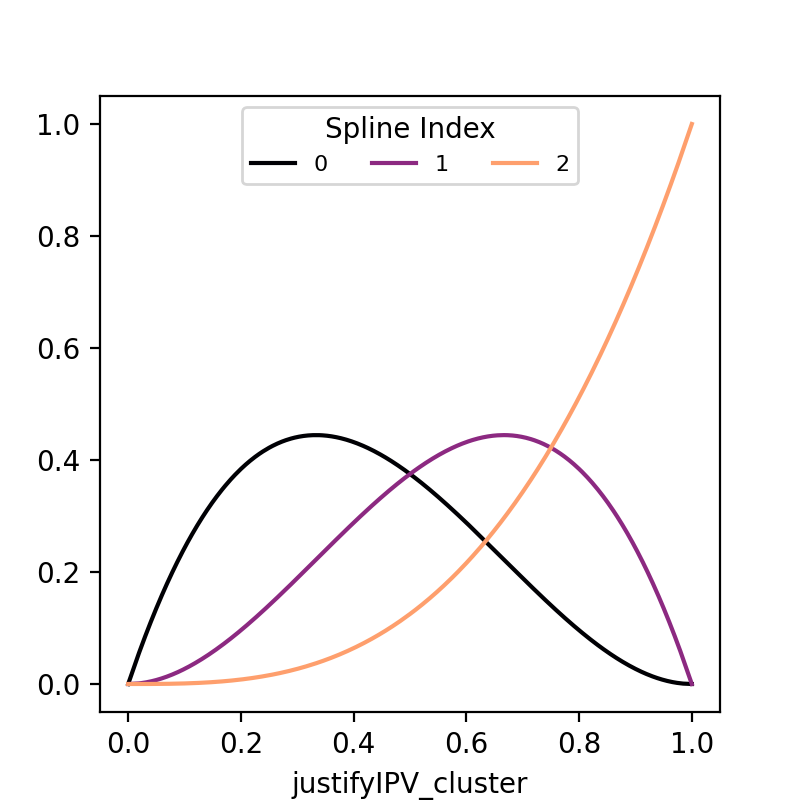
\includegraphics{figure/splines-data-preparation-inspect-spline-1.png}
  \caption{The mapping between proportion of women in the neighbourhood that thinks IPV can be justified and the splines used in model 2.}
\end{figure}

\newpage

\bibliographystyle{plain}
\bibliography{references}

\end{document}
